%%%%%%%%%%%%%%%%%%%%%%%%%%%%%%%%%%%%%%%%%%%%%%%%%%%%%%%%%%%%%%%%%%%%%%%%
% 
% LaTeX Template
%
%%%%%%%%%%%%%%%%%%%%%%%%%%%%%%%%%%%%%%%%%%%%%%%%%%%%%%%%%%%%%%%%%%%%%%%%

%------------------------------------------------------------------------------------------------
%	DOCUMENT CONFIGURATIONS
%------------------------------------------------------------------------------------------------

% DOCUMENT
%   - Properties
\documentclass[a4paper,11pt]{report} % Sets a two-sided A4 sized paper.
                                         % (Two-sided for LaTeX to distinguish between odd/even
                                         % pages while using headers and footers.)
\linespread{1.15}                         % Default space between lines
                                    % Margin sizes defined in headers_and_footers file.
\usepackage[nottoc,numbib]{tocbibind}    % Makes References section appear in the Table of contents (nottoc). Conuts the References like section.
\usepackage{lastpage}                    % To get the total number of pages.

%   - Sectioning
\usepackage{titlesec}                   % Extra features for sectioning
    % The following lines create: \subsubsubsection{}
    
    
%%%%%%%%% From here: creation of \subsubsubsection{} %%%%%%%%%
    \titleclass{\subsubsubsection}{straight}[\subsection]

    \newcounter{subsubsubsection}[subsubsection]
    \renewcommand\thesubsubsubsection{\thesubsubsection.\arabic{subsubsubsection}}
    \renewcommand\theparagraph{\thesubsubsubsection.\arabic{paragraph}} % optional; useful if paragraphs are to be numbered

    \titleformat{\subsubsubsection}
      {\normalfont\normalsize\bfseries}{\thesubsubsubsection}{1em}{}
    \titlespacing*{\subsubsubsection}
    {0pt}{3.25ex plus 1ex minus .2ex}{1.5ex plus .2ex}

    \makeatletter
    \renewcommand\paragraph{\@startsection{paragraph}{5}{\z@}%
      {3.25ex \@plus1ex \@minus.2ex}%
      {-1em}%
      {\normalfont\normalsize\bfseries}}
    \renewcommand\subparagraph{\@startsection{subparagraph}{6}{\parindent}%
      {3.25ex \@plus1ex \@minus .2ex}%
      {-1em}%
      {\normalfont\normalsize\bfseries}}
    \def\toclevel@subsubsubsection{4}
    \def\toclevel@paragraph{5}
    \def\toclevel@paragraph{6}
    \def\l@subsubsubsection{\@dottedtocline{4}{7em}{4em}}
    \def\l@paragraph{\@dottedtocline{5}{10em}{5em}}
    \def\l@subparagraph{\@dottedtocline{6}{14em}{6em}}
    \makeatother

    \setcounter{secnumdepth}{4}
    \setcounter{tocdepth}{4}
%%%%%%%%% Until here: creation of \subsubsubsection{} %%%%%%%%%


%\let\oldsection\section % This line and the following force sections to start on odd pages.
%\def\section{\cleardoublepage\oldsection}

\newcommand*{\blankpage}{%
    \vspace*{\fill}
        \begin{center}
            (This page was intentionally left in blank.)
        \end{center}
    \vspace{\fill}
}
\makeatletter
\renewcommand*{\cleardoublepage}{\clearpage\if@twoside \ifodd\c@page\else
\blankpage
\thispagestyle{empty}
\newpage
\if@twocolumn\hbox{}\newpage\fi\fi\fi}
\makeatother

% WRITING
%   - Math/Chemistry/...
\usepackage{amsmath}                % Mathematical features.
    % Section numbering
    \numberwithin{equation}{section}    % Equation numbering by section
    \numberwithin{table}{section}       % Table numbering by section
    \numberwithin{figure}{section}      % Table numbering by section
\usepackage{amssymb}                % Symbols.
\usepackage[version=3]{mhchem}                 % Chemical equation typesetting. i.e.: \ce{CO2 + C <=> 2CO}
\usepackage{siunitx}                % Simplifies the usage of values with units.
                                    % i.e.: "\SI{5.4}{kg·m^{-1}·s^{-2}}"
                                    % instead of "5.4 kg·m$ ^{-1} $·s$ ^{-2} $"
\usepackage{eurosym}                % Use EURO symbol (\euro)

%%   - Language
\usepackage[utf8]{inputenc}         % Required for the usage of characters like 'ñ', 'ú', ...
%\renewcommand{\figurename}{Figura}  % In captions, print "Figura" (in Catalan) instead of
                                    % "Figure" (English default name).
%\renewcommand{\tablename}{Tabla}
%\renewcommand{\contentsname}{Índice}
%\renewcommand{\refname}{Bibliografía}

%   - Text
%\let\oldsection\section             % This line and the nextone force sections to start always in new odd pages.
%\def\section{\cleardoublepage\oldsection} %
\usepackage[none]{hyphenat}         % [none] Prevents any hyphenation throughout the document.
                                    % (hyphenation -> "separació per síl·labes")
\sloppy                             % Forces wrapping at word boundaries by relaxing the interword space constraints.
%\usepackage{indentfirst}            % Forces indentation from paragraphs after a section.
                                    % (see notes 1 and 2)
\setlength\parindent{1cm}           % Removes all indentation from paragraphs.
%\newenvironment{paragraphs}{\setlength\parindent{1cm}}{\setlength\parindent{0cm}}
                                    % "\begin{paragraphs}" will create an environment where
                                    % indentation from paragraphs is activated.
\usepackage[font=footnotesize]{caption} % Captions
\setlength{\abovecaptionskip}{0pt}      %
\setlength{\belowcaptionskip}{0pt}      %
\usepackage{lmodern}                % Allow the use of font size larger tha 25pt
\usepackage[T1]{fontenc}            %

% GRAPHICS, TABLES AND OTHERS
\usepackage{graphicx}               % Required for the inclusion of images.
\usepackage{float}                  % Required for some float properties.
\usepackage{pdfpages}               % Required for the inclusion of PDF files.
\usepackage{multirow,longtable,array,booktabs,tabularx} % More features for tables.
\usepackage{enumerate}              % Gives the enumerate environment an optional argument which
                                    % determines the style in which the counter is printed.
\usepackage{enumitem}               % Extra options for "enumerate" lists
\usepackage{color}                  % Use some color options.
\usepackage{colortbl}               % Use some other color options.
	\definecolor{UPC_blue}{RGB}{67,142,197}
	\definecolor{lightgrey}{RGB}{166,166,166}
\usepackage{hyperref}               % Provides LeTeX the hability to create hyperlinks.

\usepackage{inputenc}         % It makes possible to use roman numbers for the pages before the first chapter and arabic for the rest of the document

\usepackage{booktabs}
\usepackage{xcolor,colortbl}
\usepackage{pstricks}
\usepackage{blindtext}
\usepackage{transparent}
\usepackage{etoolbox}
\usepackage{pdflscape}
\usepackage{amsmath}
\usepackage{amsfonts}
\usepackage{amssymb}
\usepackage{graphicx}
\usepackage{eurosym}
\usepackage{wrapfig}
\usepackage{mathdots}
\usepackage{caption}
\usepackage{cite}
\usepackage{mathrsfs}
\usepackage{float}
\usepackage{import}
\usepackage{makecell}
\usepackage{booktabs}
\usepackage{caption}
\usepackage{subcaption}
\usepackage{textcomp}

%   - NOTES
% (1) LaTeX implements a style that doesn't indent the first paragraph after a section heading. There are coherent reasons for this. Some typography rules state that first indent should be suppressed only after a centered title and that all other paragraphs must be indented.
% (2) We have already removed all indentation from paragraphs with the command "\setlength\parindent{0cm}", but when using the environment we've created "escrit" we set indent to 1cm. Then, if this environment is used right after a section the first indent will be suppressed unless we use the package "indentfirst". % Document Configurations

%-----------------------------------------------------------------------------
%	REPORT INFORMATION
%-----------------------------------------------------------------------------

%%% MAIN INFORMATION %%%

% School
\newcommand{\School}{ESEIAAT}
\newcommand{\researcherDept}{Airports design and construction}
% Degree
\newcommand{\Degree}{Master's degree in Aerospace Engineering}

% Department
\newcommand{\Department}{Airports design and construction}

% Secció (Secció de Terrassa)
\newcommand{\Seccio}{Secció de Terrassa}

% Course
\newcommand{\Course}{220304 - Airports design and construction}

% Students (if you don't use that much students, leave them in blank)
\newcommand{\Studi}	{Fontanes Molina, Pol}

% Customer:
\newcommand{\Director}{Montanyà Puig, Joan}
\newcommand{\CoDirector}{Williams, Earle}

% Project Name
\newcommand{\ProjectName}{BEKASI-EAST JAKARTA AIRPORT}

% Acronym
\newcommand{\Acronym}{AIR SIDE}

% Short Name
\newcommand{\ShortName}{Director Plan}

% Kind of document
\newcommand{\DocType}{Report}

% Page number preceding (leave in blank if nothing is required)
% Suggestion: R, RA, B, D, T referred to report, report attachments, budget, drawings or technical sheets
\newcommand{\precPage}{R}


% Date of the document (Delivery date)
	% Day
	\newcommand{\DocDateD}{10}
	% Month
	\newcommand{\DocDateM}{12}
	% Year
	\newcommand{\DocDateY}{2017}

%-----------------------------------------------------------------------------
% Don't touch this unless you know what you are doing!

% Generation of Group Code
\newcommand{\GrCode}{{\GrNum} EA-\GrTerm\GrYr} 

% Generation of the date format
\newcommand{\DocDate}{\DocDateD-\DocDateM-\DocDateY}  % Document information

%-----------------------------------------------------------------------------
%	HEADERS AND FOOTERS
%-----------------------------------------------------------------------------

% Changes default margins.
\usepackage[left=3cm,right=3cm,top=2.5cm,bottom=2.5cm]{geometry}
   \setlength{\headheight}{50pt}         % Header Space.
   \setlength{\textheight}{640pt}        % Text height.
   \setlength{\footskip}{30pt}           % Foot Space.

\usepackage{fancyhdr}
	\pagestyle{fancy} % Headers and footers -> "fancy" style.
	
	% Obtain the name of the section:
	\renewcommand{\sectionmark}[1]{\markright{Section \thesection : #1}}
	\renewcommand{\chaptermark}[1]{\markleft{Chapter \thechapter : #1}} 

	\fancyhf{} % Clear all headers and footers fields

% Package info and examples
%		% O/E = Odd/Even page // L/C/R = Left/Center/Right field
%	\fancyhead[LE]{\hspace{-10pt}
%		\raisebox{-\height+12pt}{
%		
\includegraphics[height=30pt]{./doc_config/images/UPC_dpt}
%		}
%	}
%	\fancyhead[RE]{\bf \Department}
%	\fancyhead[LO]{\bf \DocType}
%	\fancyhead[RO]{\bf \emph{\ProjectName}}
%	\fancyfoot[LE,RO]{\thepage} % Adds customized pages numbers



%-----------------------------------------------
% General headers and footers of the document:
%-----------------------------------------------
	% Headers
	\fancyhead[LO]{\textbf{\rightmark}} % Section mark
	\fancyhead[RO]{
\includegraphics[height=25pt]{./doc_config/images/logo}}
	\fancyhead[LE]{\textbf{\rightmark}}
	\fancyhead[RE]{
\includegraphics[height=25pt]{./doc_config/images/logo}}

	% Footers
	\fancyfoot[CE,CO]{\precPage{} - \thepage}
	\fancyfoot[LO,RE]{\textbf{\Acronym}}

	\renewcommand{\headrulewidth}{0.5pt} % Header decorative line
	\renewcommand{\footrulewidth}{0.5pt} % Footer decorative line
	\renewcommand{\chaptermark}[1]{%
\markboth{#1}{}}
\renewcommand{\sectionmark}[1]{\markright{#1}}


%-----------------------------------------------
% Headers and footers for pages where chapter starts:
%-----------------------------------------------
\fancypagestyle{plain}{
	%Headers
	\fancyhead[LO]{\textbf{\leftmark}} % Section mark
	\fancyhead[RO]{
\includegraphics[height=25pt]{./doc_config/images/logo}}
	\fancyhead[LE]{\textbf{\leftmark}}
	\fancyhead[RE]{
\includegraphics[height=25pt]{./doc_config/images/logo}}
	%Footers
	\fancyfoot[CE]{\precPage{} - \thepage}
	\fancyfoot[CO]{\precPage{} - \thepage}
	\fancyfoot[LO,RE]{\textbf{\Acronym}}
	
	\renewcommand{\headrulewidth}{0.5pt} % Header decorative line
	\renewcommand{\footrulewidth}{0.5pt} % Footer decorative line
}


%-----------------------------------------------
% Cover headers and footers:
%-----------------------------------------------

	\fancypagestyle{CoverPage}{ % This creates a new headers and footers page style.
	                            % To use it type "\thispagestyle{FirstPage}" on the first page.
	                                % (right after "\maketitle")
		\fancyhf{}
		%\fancyfoot[C]{Group \GrCode \hfill [\DocDate]}
		\renewcommand{\headrulewidth}{0pt}
		\renewcommand{\footrulewidth}{0pt}
	}


%-----------------------------------------------
% No headers nor footers page (ie: Back cover)
%-----------------------------------------------

	\fancypagestyle{EmptyPage}{
		\fancyhf{}
		\renewcommand{\headrulewidth}{0pt}
		\renewcommand{\footrulewidth}{0pt}
	} % Headers and footers

%-----------------------------------------------------------------------------
%	USER DEFINED ENVIRONMENTS
%-----------------------------------------------------------------------------

% Itemize with reduced vertyical space between items
\newenvironment{itemize_rvs}
{ \begin{itemize}
    \setlength{\itemsep}{0pt}
    \setlength{\parskip}{0pt}
    \setlength{\parsep}{0pt}     }
{ \end{itemize}                  }

% Standard names

% Titles and sections structures
\newcommand{\subpart}[1]{\mbox{ }\\\noindent\textbf{#1}}
\newcommand{\subsubpart}[1]{\mbox{ }\\\indent\underline{#1}}
\newcommand{\subsubsubpart}[1]{\mbox{ }\\\indent\indent\textit{#1}}

% Figure/table source
\newcommand{\source}[1]{\caption*{\hfill Source: {#1}} } % User defined environments

% Paragraph formatting
\setlength{\parindent}{0pt}

\usepackage{textcomp}
\usepackage{gensymb}
\usepackage{epigraph}
\usepackage{tocloft}
\usepackage{multicol}
\usepackage[T1]{fontenc}
\usepackage{titlesec, blindtext, color}
\definecolor{gray75}{gray}{0.75}
\newcommand{\hsp}{\hspace{20pt}}
\titleformat{\chapter}[hang]{\Huge\bfseries}{\thechapter\hsp\textcolor{gray75}{|}\hsp}{0pt}{\Huge\bfseries}

\renewcommand{\familydefault}{\sfdefault}

\begin{document}

%-----------------------------------------------------------------------------
%	Project Charter Cover
%-----------------------------------------------------------------------------

\thispagestyle{CoverPage}

% Centered cover page

\begin{center}\bf


\includegraphics[width=0.2\textwidth]{./doc_config/images/logo.png}\\
%\large \researcherDept

\vspace{50pt}

%{\large \School}

\vspace{6pt}


\includegraphics[width=0.6\textwidth]{./doc_config/images/UPC_ESEIAAT.jpg}

\vspace{50pt}

%{\Huge \ProjectName}\\
{\fontsize{24pt}{20pt}\selectfont \ProjectName}

\vspace{10pt}

{\fontsize{20pt}{20pt}\selectfont \Acronym}

%\includegraphics[width=0.4\textwidth]{./doc_config/images/DF_logo}

\textcolor{UPC_blue}{\rule{\textwidth}{.6pt}}

{\Large \DocType}

\end{center}

\vspace{50pt}

\textbf{Degree:} \Degree

\textbf{Course:} \Course

\textbf{Delivery date:} \DocDate\\

\vspace{10pt}

%\textbf{Students:} \Studi
\textbf{Students:} Abiétar Moreno, Sergi; Delgado Chicote, Miguel; Fernández Porta, Sergi; Fernández Sanz, Sergio; Fontanes Molina, Pol and Vidal Pedrola, Xavier

%\textbf{Director:} \Director

%\textbf{Co-Director:} \CoDirector % COVER
\newpage\thispagestyle{EmptyPage}
\mbox{}\newpage

\pagenumbering{roman}

% TABLE OF CONTENTS
\setcounter{tocdepth}{3}
\tableofcontents
\pagebreak

%\mbox{}\newpage
\renewcommand{\cfttabnumwidth}{4em}
\listoftables
\pagebreak

%\mbox{}\newpage
\renewcommand{\cftfignumwidth}{4em}
\listoffigures


% DOCUMENT SECTIONS

\newpage
\pagenumbering{arabic}

\newpage
\setlength{\parskip}{1em}

\chapter{Airport location and characterization}

	\section{Location}

	\section{Meteorology}
		\subsection{Temperature}
		\subsection{Wind}
\chapter{Runway design}

	\section{Introduction}
	\paragraph{} The runway is a key piece of the airport and the air side design due to the fact that defines the maximum dimensions of the operative air planes. Its function is to successfully guarantee the landing and takeoff operation.
	
	In order to successfully define the runway, the instructions and requirements given in the Annex 14 given by the ICAO have been followed. 

	\section{Runway Length}
	\paragraph{} The reference field length is defined as the minimum distance needed in order to perform a takeoff operation with the maximum homologated takeoff weight using sea level conditions, without wind and considering 0° slope.  

	In order to calculate the runway length, the first step is to choose the most restrictive air plane that is going to operate on that runway. Afterwards, that length has to be corrected by the runway slope, the altitude of the airport and the mean temperature.

	Due to the fact that the airport has two runways, from now on, the runway used for international flights will be referred as runway 1 and the one used for domestic flights will be named runway 2. 
	
		\subsection{Runway 1}
		The biggest airplanes that will operate on this runway are the Boeing 777-300ER and the Airbus A330-300. 
		
			\subsubsection{Reference Field Length}
			Starting with the B777-300ER, using the ACAP (Aircraft Characteristic for Airport Planning), the values of the MTOW (Maximum TakeOff Weight) and MLW (Maximum Landing Weight) can be obtained. 
			
			\begin{figure}[H]
				\centering
				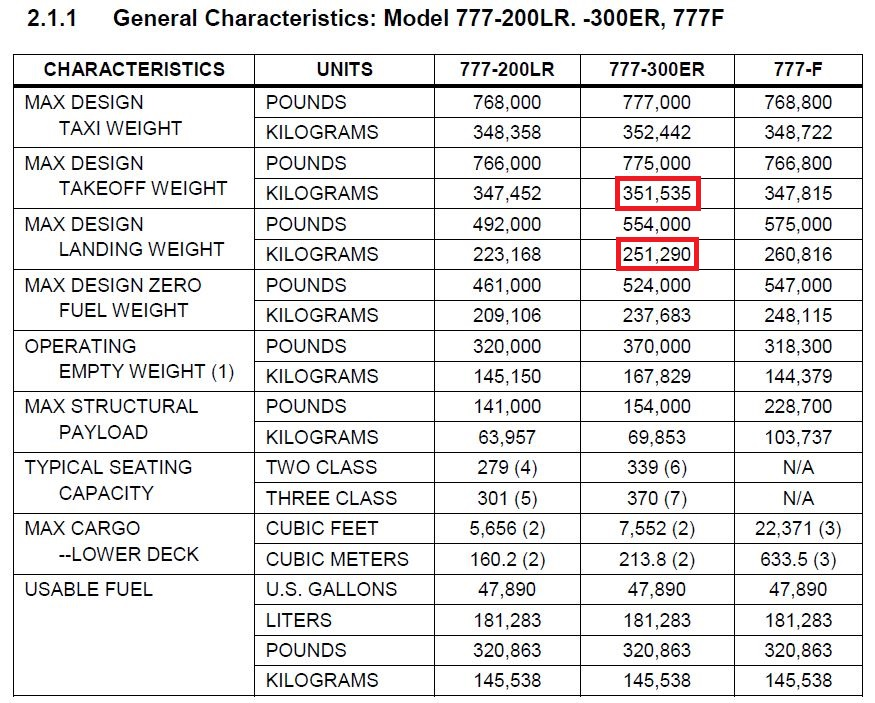
\includegraphics[clip, trim=0cm 0cm 0cm 0cm, width=1\textwidth]{./images/B777/B777MTOW}
				\caption{Maximum weights of the B777 depending on its configuration.} %nom de la figura
				\label{} %per denotar una referencia
			\end{figure}

			The next step is to calculate using the following graph the takeoff distance required with standard day + 15ºC = 30ºC and sea level conditions.
			
			\begin{figure}[H]
				\centering
				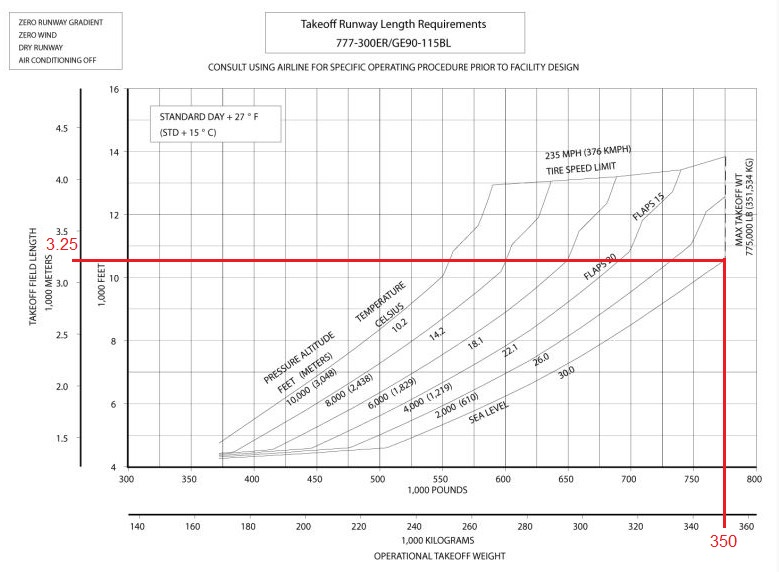
\includegraphics[clip, trim=0cm 0cm 0cm 0cm, width=1\textwidth]{./images/B777/payload-takeoffdistance}
				\caption{Relation between the MTOW and the takeoff distance.} %nom de la figura
				\label{} %per denotar una referencia
			\end{figure}
			
			As it is seen on the graph above, the length taken as reference (LCR) is 3.250m in a standard day+15ºC and sea level conditions. 
			
			The same procedure has to be done with the Airbus A330-300 in order to compare which one is the most restrictive one. Using the ACAP (Aircraft Characteristic for Airport Planning), the MTOW and MLW obtained are the following:
			
			\begin{figure}[H]
				\centering
				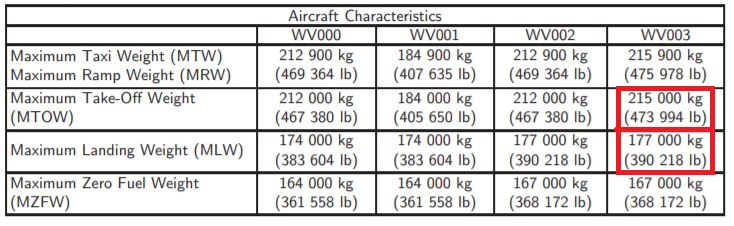
\includegraphics[clip, trim=0cm 0cm 0cm 0cm, width=1\textwidth]{./images/A330/A330}
				\caption{Maximum A330's weights.} %nom de la figura
				\label{} %per denotar una referencia
			\end{figure}
			
			Since the difference on the MTOW and MLW between both planes is greater than a 50\%, the Boeing’s Reference Field Length is chosen as the critical without calculating the Reference Field Length of the A330-300.
			
			Once the most restrictive plane is chosen, the next step is to correct the length following ICAO’s instructions. The equation used to correct the altitude difference is:
			
			\[L_t=RFL*(1+0,07*\frac{\Delta h}{300})\]
			
			Solving the equation for a RFL of 3.250m and an increase on the altitude of 100m, the result obtained is 3326m.
			Since the temperature has already been corrected on the graph and the runway slope is going to be less than 0,5\% and thus, it can be neglected, the final length will be 3.500m rounding up.
		
			\subsubsection{Reference code}
			Using the dimensions of the B777-300ER and the tables given by the ICAO, the number and letter that define the runway can be obtained. 
			
			\begin{figure}[H]
				\centering
				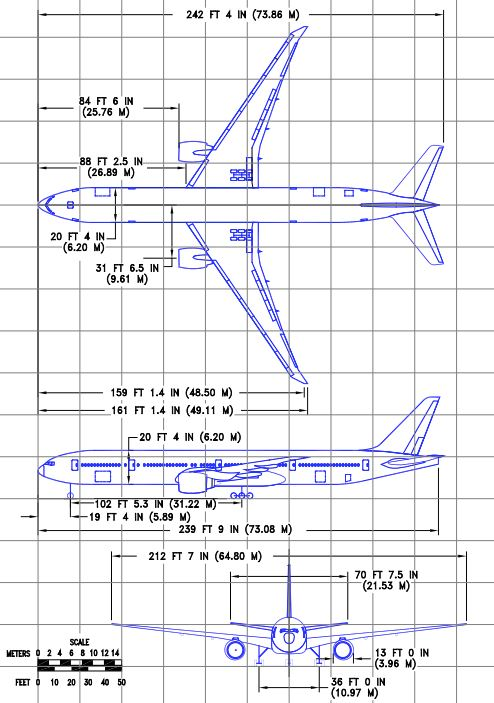
\includegraphics[clip, trim=0cm 0cm 0cm 0cm, width=1\textwidth]{./images/B777/Dimensions777}
				\caption{Boeing 777-300ER dimensions.} %nom de la figura
				\label{} %per denotar una referencia
			\end{figure}
				
			\begin{figure}[H]
				\centering
				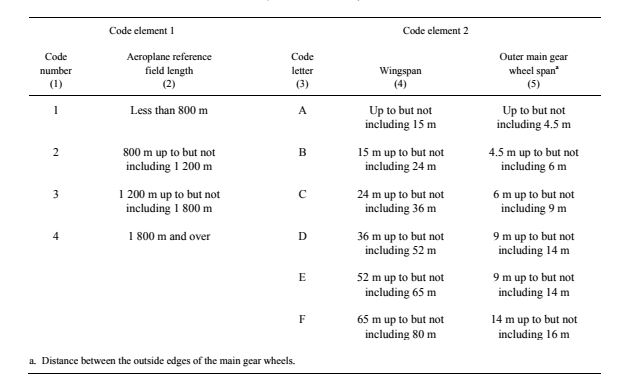
\includegraphics[clip, trim=0cm 0cm 0cm 0cm, width=1\textwidth]{./images/Annex14/Referencecode}
				\caption{Reference code given by the ICAO.} %nom de la figura
				\label{} %per denotar una referencia
			\end{figure}
		
			\paragraph{}Due to the RFL being higher than 1800m , the reference number of the runway is number 4 according to ICAO and due to the dimensions of the air plane B777-300ER, which has a span of 64,8m<65m and a distance between the landing gear of 10,97m<14m, the letter that defines the airport is E.
			
			\subsubsection{Runway width and shoulders}
			\paragraph{}The runway width is obtained using the ICAO recommendations stated on the Annex 14 and the key reference of the runway. 
			
			\begin{figure}[H]
				\centering
				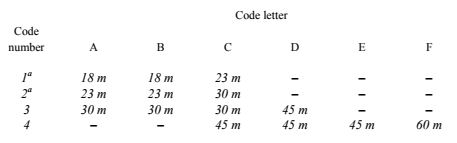
\includegraphics[clip, trim=0cm 0cm 0cm 0cm, width=1\textwidth]{./images/Annex14/RunwayWidth}
				\caption{Runway width according to OACI.} %nom de la figura
				\label{} %per denotar una referencia
			\end{figure}
		
			As it can be seen, and remembering that our key reference is 4E, the minimum runway width needed is 45m. This value has to be further increased with the use of runway shoulders up to a minimum of 60m. 

			\subsubsection{Declared distances}
			\paragraph{} The calculations done in order to obtain the final value can be seen on the airside’s attachments section 1. 
			
			To sum up, the final values obtained are:
			
			\subsubsection{Runway strips}
			\subsubsection{Runway end safety area (RESA)}
			\subsubsection{Stopway (SWY)}
			\subsubsection{Clearway (CWY)}
			
		\subsection{Runway 2}
		In this case, the planes that are going to be evaluated are the Boeing 737-800 and the Airbus 320-200.
		\subsubsection{Reference Field Length}
		Searching the values of MTOW and MLW stated on the ACAP of the Boeing 737, the values obtained are 79.000kg for the MTOW and 66.300kg for the MLW.
		
		\begin{figure}[H]
			\centering
			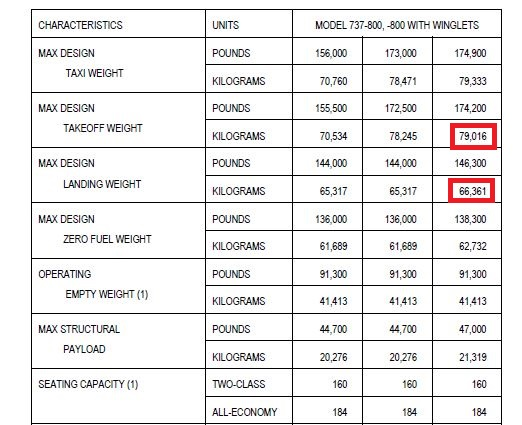
\includegraphics[clip, trim=0cm 0cm 0cm 0cm, width=1\textwidth]{./images/B737/B737MTOW}
			\caption{Maximum weights of the B737 depending on its configuration.} %nom de la figura
			\label{} %per denotar una referencia
		\end{figure}
	
		As for the B777, the next step is to calculate using the following graph the takeoff distance required with standard day + 15ºC = 30ºC and sea level conditions using the MTOW.
		
		\begin{figure}[H]
			\centering
			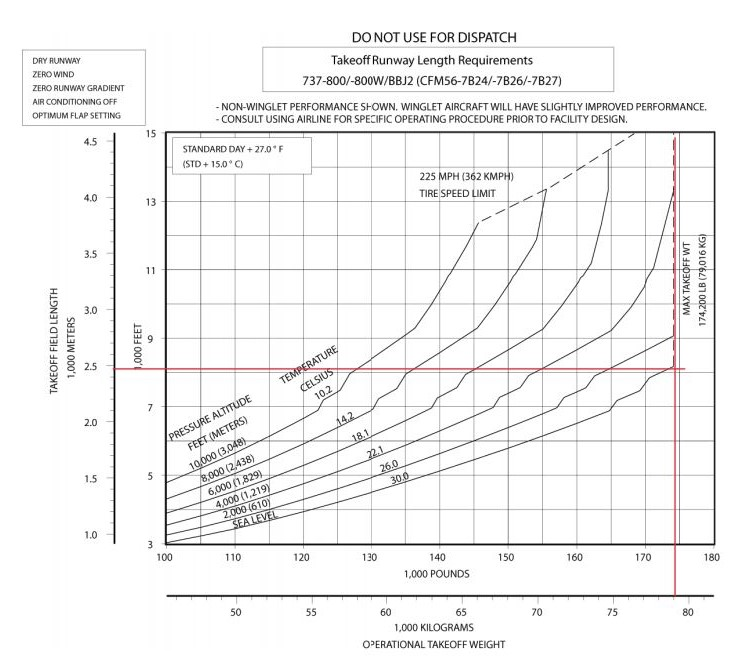
\includegraphics[clip, trim=0cm 0cm 0cm 0cm, width=1\textwidth]{./images/B737/takeoff-weight737}
			\caption{Relation between the MTOW and the takeoff distance.} %nom de la figura
			\label{} %per denotar una referencia
		\end{figure}
	
		The value of the RFL obtained is 2.450m approximately in standard day and sea level conditions. 
		
		The same procedure has to be done with the Airbus A320-200 in order to compare which one is the most restrictive one. Using the ACAP (Aircraft Characteristic for Airport Planning), the MTOW and MLW obtained are the following:
		
		\begin{figure}[H]
			\centering
			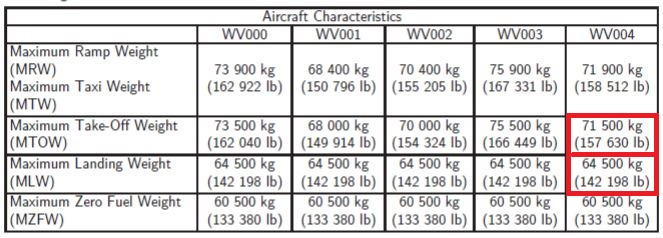
\includegraphics[clip, trim=0cm 0cm 0cm 0cm, width=1\textwidth]{./images/A320/A320MTOW}
			\caption{Maximum weights of the A320 depending on its configuration.} %nom de la figura
			\label{} %per denotar una referencia
		\end{figure}
	
		Due to the fact that the MTOW and the MLW of the B737 are higher than the A320 ones, the plane B737 is chosen as the critical for the design of the runway. 		
		
		The next step is to correct the field length using the equation stated above, on the calculations for runway 1. 
	
		\[L_t=RFL*(1+0,07*\frac{\Delta h}{300})\]
		
		Solving the equation for a RFL of 2.450m and an increase on the altitude of 100m, the result obtained is 2500m.
		The same hypotheses used on the runway number 1 will be applied regarding the temperature and slope of the runway.  Thus, the final length will be 2500m.
		
		\subsubsection{Reference code}
		Using the dimensions of the B737-800 and the tables given by the ICAO, the number and letter that define the runway can be obtained. 
		
		\begin{figure}[H]
			\centering
			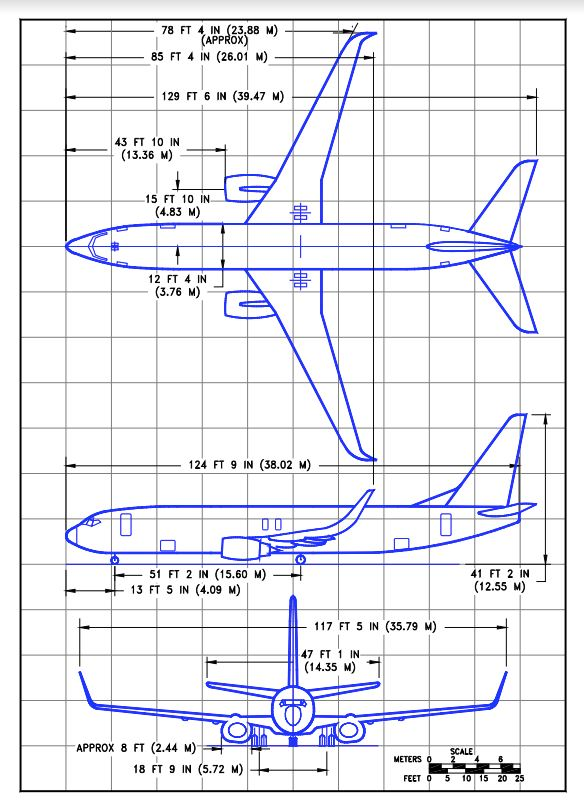
\includegraphics[clip, trim=0cm 0cm 0cm 0cm, width=1\textwidth]{./images/B737/737}
			\caption{Boeing 737-800 dimensions.} %nom de la figura
			\label{} %per denotar una referencia
		\end{figure}
	
	\paragraph{}Due to the RFL being higher than 1800m , the reference number of the runway is 4 according to ICAO and due to the dimensions of the air plane B737-800, which has a span of 35,8m<36m and a distance between the landing gear of 6m<9m, the letter that defines the airport is C.
	
	\subsubsection{Runway width and shoulders}
	\paragraph{}The runway width is obtained using the ICAO recommendations stated on the Annex 14 and the key reference of the runway. 
	
	\begin{figure}[H]
		\centering
		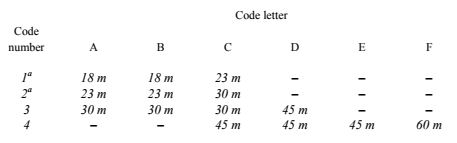
\includegraphics[clip, trim=0cm 0cm 0cm 0cm, width=1\textwidth]{./images/Annex14/RunwayWidth}
		\caption{Runway width according to OACI.} %nom de la figura
		\label{} %per denotar una referencia
	\end{figure}
	
	As it can be seen, and remembering that our key reference is 4C, the minimum runway width needed is 45m. This value has to be further increased with the use of runway shoulders up to a minimum of 60m. 
	
		\subsubsection{Declared distances}
	\paragraph{} As for the runway 1, the calculations done in order to obtain the final value can be seen on the airside’s attachments section 1. 
	
	To sum up, the final values obtained are:
	
	\subsubsection{Runway strips}
	\subsubsection{Runway end safety area (RESA)}
	\subsubsection{Stopway (SWY)}
	\subsubsection{Clearway (CWY)}
	
	
		
		
		
\chapter{Taxiway design}
	
	\section{Introduction}
	\paragraph{}The aim of the taxiways is to link the different parts of the airport such as the different runways, the terminal, hangars or the parking lot. Several factors must be taken into account when designing this part of the airside; it goes without saying that this design must make the operations easy, efficient and must minimise the total amount of crosses in the flows and in the traffic.
	
	\section{Taxiway's width}
	\paragraph{}OACI’s Annex 14 states that, depending of the code letter, the width must be, at least:
	
	\begin{table}[htb]
		\centering
		\begin{tabular}{ll p{5cm}}
			\toprule[2pt]
			Code letter & Taxiway width [m]\\
			\midrule[1pt]
			A & 7,5\\
			B & 10,5 \\
			C & 15\\
			D & 18-23\\
			E & 23\\
			F & 25\\
			\bottomrule[2pt]
		\end{tabular}
		\caption{Taxiway width depending on its code letter.}
		\label{}
	\end{table}
	
	Due to the fact that our airport has 2 different runways, thus, two different code letters. Thus, the international runway will have a taxiway of 23m since its code letter is E and the domestic one will have 15m since its category is C.
	
	\section{Taxiway's turns}
	\paragraph{}Even though it is recommended that the fewer changes in direction, the better, the Annex 14 stipulates that, for a plane that remains over the taxiway centre line markings, the distance between the outer main wheel and the edge of the taxiway should be, at least:
	
	\begin{table}[htb]
		\centering
		\begin{tabular}{ll p{5cm}}
			\toprule[2pt]
			Code letter & Clearance [m]\\
			\midrule[1pt]
			A & 1,5\\
			B & 2,25 \\
			C & 3-4,5\\
			D & 4,5\\
			E & 4,5\\
			F & 4,5\\
			\bottomrule[2pt]
		\end{tabular}
		\caption{Clearance depending on its code letter.}
		\label{}
	\end{table}

	For the international runway, the clearance will be 4,5m and 3m for the domestic flights runway.
	
	\section{Minimum separation distance}
	\paragraph{}Taking the axis of the taxiway and the axis of the runway or any other taxiway as the reference elements of both paths, under no circumstances should the distance between them be less than the ones shown in table 3.1 in Annex 14 (unless an existing minor distance is proven not to affect negatively the security of the system).
	
	\section{Taxiway's slope}
	\paragraph{}In this section, the taxiway's slope will be boarded, trying to bring solutions in case that the slope can't be changed. 
		\subsection{Longitudinal slope}
		\paragraph{}The longitudinal slope of a taxiway should never exceed:
		
		-	1,5\% if the code letter is C, D, E or F.
		
		-	3\% if the code letter is A or B.
		
		Even though the longitudinal slope has to be tried to be reduced to a minimum, the final longitudinal slope will be 1\% on each runway.
				
		\subsection{Change of the longitudinal slope}
		\paragraph{}If it is not possible to prevent the change of the slope in a taxiway, the transition among them should be a curved surface which curvature should not exceed:
		
		-	1\% for every 30m (radius of curvature approximately 3.000 m) if the code letter is C, D, E or F.
		
		-	1\% for every 25m (radius of curvature approximately 2.500 m) if the code letter is A or B.
	
		Since the longitudinal slope is within the limits established by the ICAO's recommendations, there is not going to be any local change of the longitudinal slope.
		
		\subsection{Visible distance}
		\paragraph{}If changing the slope patterns in a taxiway is not possible, the change in slope should be the one that, from a point situated in:
	
		-	3 m above the taxiway, it could be possible to see a surface of 300 m if the code letter is C, D E or F.
	
		-	2 m above the taxiway, it could be possible to see a surface of 200 m if the code letter is B.
	
		-	1,5 m above the taxiway, it could be possible to see a surface of 150 m if the code letter is A.
	
		\subsection{Transversal slope} 
		\paragraph{}The cross slope of a taxiway, as in runways, should be strong enough to prevent the accumulation of water in its surface, but should never be greater than:
		
		-	1,5\% if the code letter is C, D, E or F.
		
		-	2\% if the code letter is A or B.
		
		The transversal slope selected for both taxiways is 1,5\%.
	
	\section{Taxiway's shoulders}
	\paragraph{}OACI’s Annex 14 recommends that taxiways subordinated to runways with code letter C, D, E or F should be designed with symmetrical margins, in order to make the total width of the taxiway, that is to say, taxiway and margins, greater than:
	
	-	60 m if the code letter is F.
	
	-	44 m if the code letter is E.
	
	-	38 m if the code letter is D.
	
	-	25 m if the code letter is C.
	
	An additional width should be added in curves, unions and intersections.
	
	Following the recommendation shown above, the taxiway's shoulders of runway 1 will be 44m and the taxiway's shoulders of runway 2 will be 25m.
	
	
	\section{Rapid exit taxiways}
		\paragraph{}As a recommendation, a rapid-exit taxiway should be calculated with a turn radius of, at least:
		
		-	550 m if code number 3 or 4.
		
		-	275 m if code number 1 or 2.
		
		In order to make the exit possible with a wet pavement at a speed of;
		
		-	93 km/h if code number 3 or 4.
		
		-	65 km/h if code number 1 or 2.
		
		Moreover, the angle of rapid-exit taxiways should be comprehended between 45\(\degree\) and 25\(\degree\), preferably 30\(\degree\). Rapid-exit taxiways should also include a straight section in order to allow the air plane to reduce its speed. 
\chapter{Holding positions}

	\section{Introduction}
	\paragraph{} Because traffic density will be medium or heavy, holding bays will be designed. Hence, runway-holding positions will be established:
	on the taxiways, at the intersection of a taxiway and a runway and at an intersection of a runway with another runway when the former runway is part of a standard taxi-route.
	
	A runway-holding position will be established on a taxiway if the location or alignment of the taxiway is such that a taxiing aircraft or vehicle can infringe an obstacle limitation surface or interfere with the operation of radio navigation aids.
	
	All the distances declared on this section will be used on the CAD model for defining each section of the airport concerning to these measures.
	
	\section{Minimum distance from the runway centre line to a holding bay, runway-holding position or road-holding position}
	
	\begin{figure}[H]
		\centering
		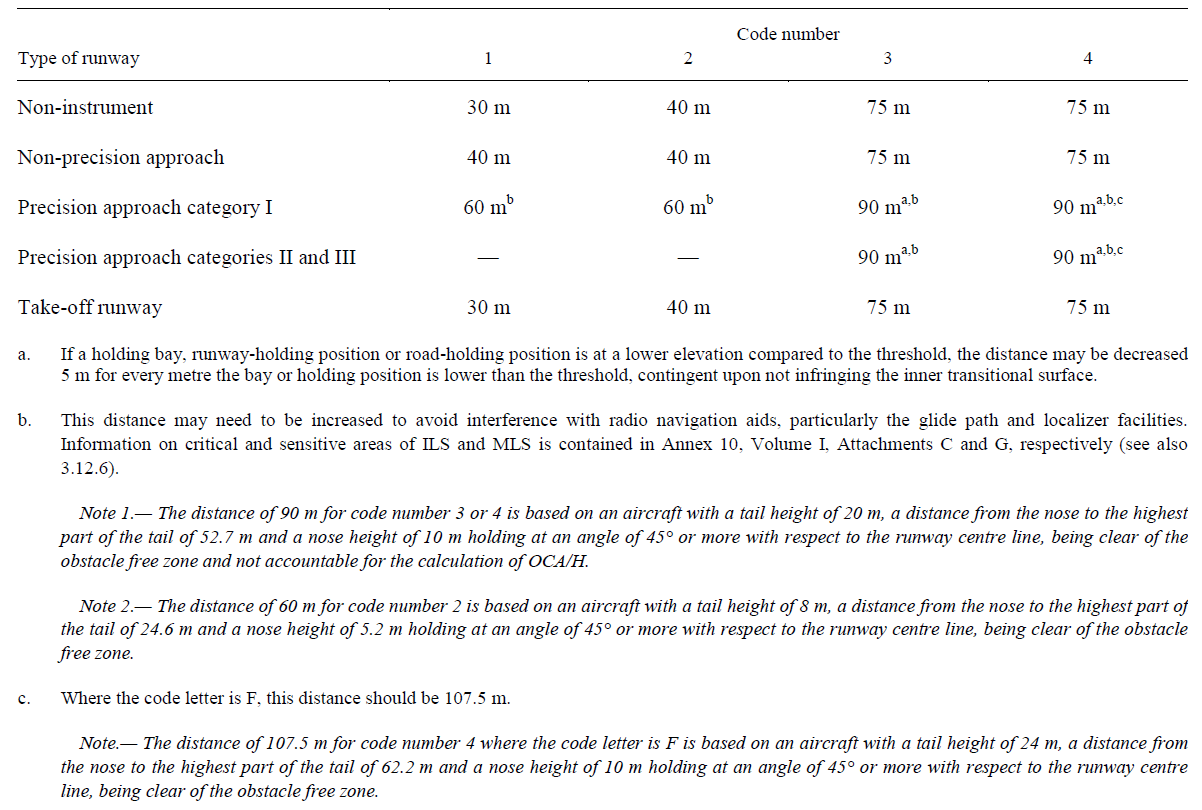
\includegraphics[clip, trim=0cm 0cm 0cm 0cm, width=1.1\textwidth]{./images/holding/distances}
		\caption{Minimum distance from the runway centre line to a holding bay, runway-holding position or road-holding position.}
		\label{distances}
	\end{figure}

	\paragraph{} Following figure \ref{distances}, minimum distances will be chosen. The location of a runway-holding position established will be such that a holding aircraft or vehicle will not infringe the obstacle free zone, approach surface, take-off climb surface or ILS/MLS critical/ sensitive area or interfere with the operation of radio navigation aids.
	
	\section{Clearance distances on aircraft stands}
	\paragraph{} An aircraft stand will provide the following minimum clearances between an aircraft entering or exiting the stand and any adjacent building, aircraft on another stand and other objects:
	
	\begin{figure}[H]
		\centering
		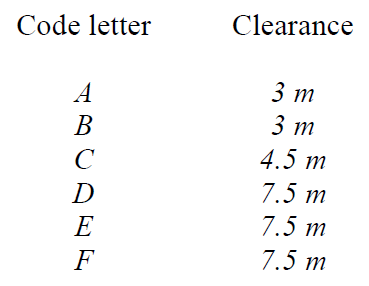
\includegraphics[clip, trim=0cm 0cm 0cm 0cm, width=0.3\textwidth]{./images/holding/clearances}
		\caption{Clearance distances on aircraft stands}
		\label{clearances}
	\end{figure}
	
	\section{Interference with critical and ILS sensible areas}
	\paragraph{} Obstacle limitation surfaces have been defined on section \textit{11. Aeronautical limitation surfaces}. Arrangements will be made to enable the appropriate authority to be consulted concerning proposed construction beyond the limits of the obstacle limitation surfaces that extend above a height established by that authority, in order to permit an aeronautical study of the effect of such construction on the operation of aeroplanes.
	
	According to the Annex 14, section 4.3, \cite{Standards2016},in this new airport, there are no obstacles interceding the ILS critical areas. From document \cite{Telecomunicaciones}, figures C-4 and AC-4B, describe how planes moving over the surface can interfere with ILS area, is not the case for the airport. It can be also corroborated in the CAD model of the whole airport. 
	
	Knowing these areas, holding positions will be collocated, properly to avoid ILS sensible areas interference. 
	
	
	\section{Interference with CWY and physical obstacles}
	
	\paragraph{} Holding points on the airport have been designed in order to avoid interfering the CWY and the RESA, while standing on the holding positions. All metrics and checks have been done on the CAD model in order to assure the viability.
	
	\section{Final design of holding positions}
	
	\paragraph{} After verifying all the holding positions regulations and also the imposed by the delivery objective. The CAT II/III holding positions have been implemented and added to the CAD drawing. Following, some details of it are shown.
		
	\begin{figure}[H]
		\centering
		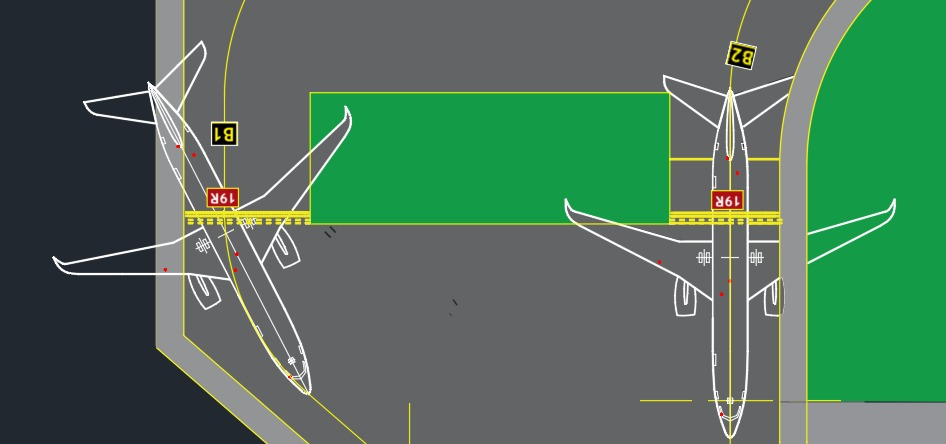
\includegraphics[clip, trim=0cm 0cm 0cm 0cm, width=\textwidth]{./images/holding/holdingRunway}
		\caption{Runway holding positions detail.}
		\label{holdingRunway}
	\end{figure}

	Note that previous figure represents the CAT II/III holding positions overview. The markings are further developed in next sections of this report, hence B1 and B2, ends up calling A and B positions respectively, as seen on figure \ref{waiting}. 

	\begin{figure}[H]
	\centering
	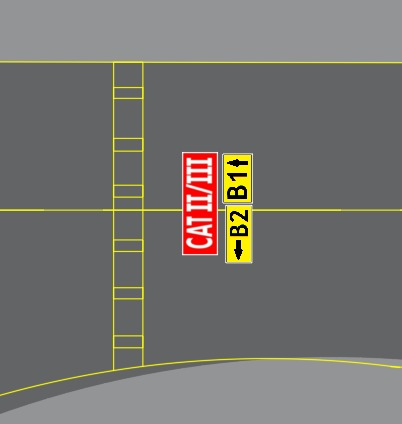
\includegraphics[clip, trim=0cm 0cm 0cm 0cm, width=0.6\textwidth]{./images/holding/cartell}
	\caption{Runway holding positions markings.}
	\label{cartell}
	\end{figure}

	\begin{figure}[H]
		\centering
		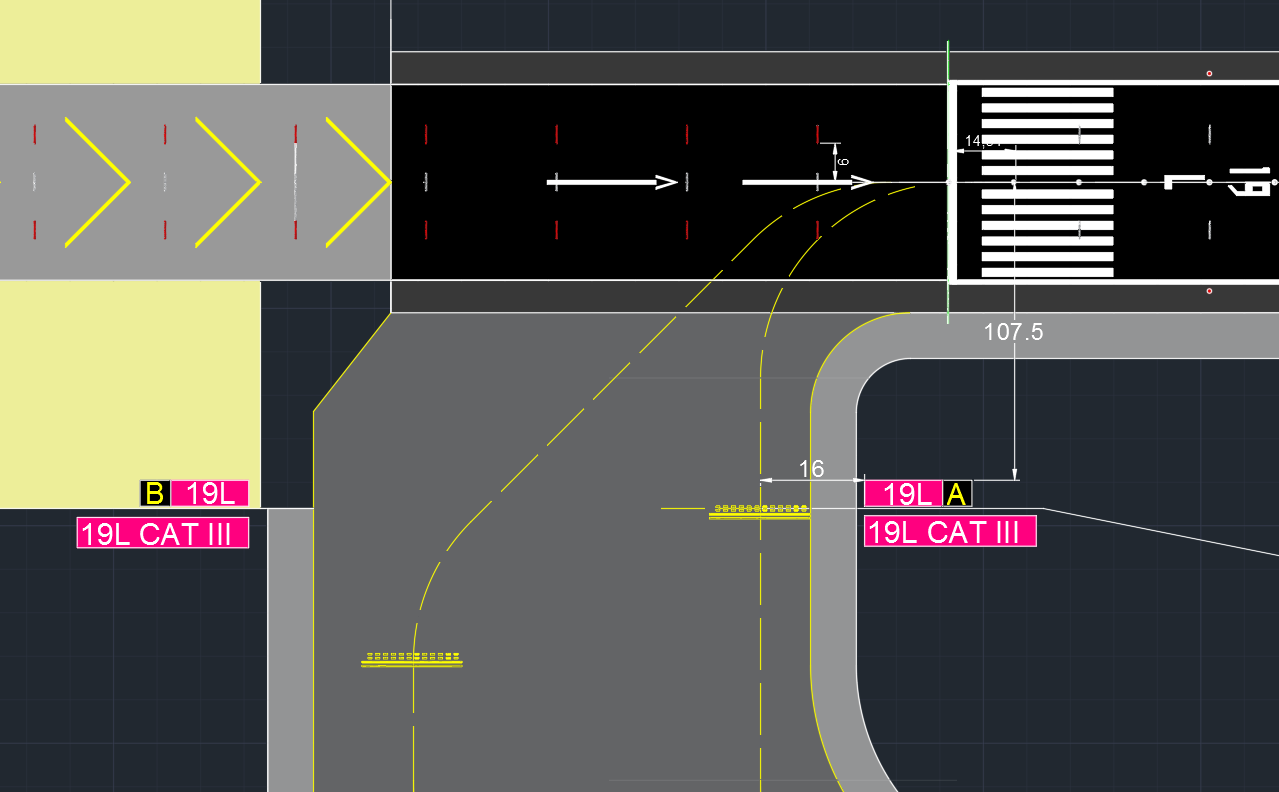
\includegraphics[clip, trim=0cm 0cm 0cm 0cm, width=0.8\textwidth]{./images/holding/waiting}
		\caption{Runway holding positions with markings.}
		\label{waiting}
	\end{figure}
	\begin{figure}[H]
		\centering
		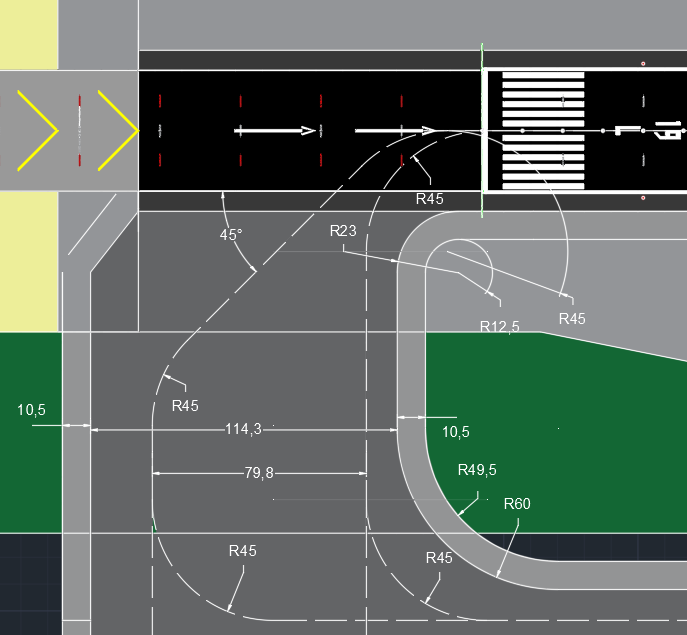
\includegraphics[clip, trim=0cm 0cm 0cm 0cm, width=0.8\textwidth]{./images/holding/sizes}
		\caption{Runway holding positions distances.}
		\label{sizes}
	\end{figure}
	
\chapter{Apron design}

	\section{Introduction}
	
	\section{Apron taxiways}
	
	\section{Aircraft stands}
		\subsection{General dimensions of aircraft stands}
		\subsection{Dimensions for reference aircraft}
		\subsection{Aircraft stands organization}
		
	\section{No equipment and holding equipment areas}
	
	\section{Apron trajectories}
	
	\section{Service ways in apron}
	
	\section{Terminal connections}
	
\chapter{Markings}
	\section{Introduction}
	\paragraph{}As a general rule, and if it is not said otherwise, in the event of an intersection, the most important way will interrupt the other ways’ central axis in order to make its own prevail. Apart from the most obvious classification, the hierarchy will be:
	
	-	Precision approximation runways
	
	-	Normal approximation runways
	
	-	Visual flight runways
	
	\underline{\textbf{\textit{Colours of the markings}}}
	
	Runway: The colour used in the marking of the runway will be white. They can be surrounded by dark markings in order to increase their visibility.
	
	Taxiway, apron and turn runway platforms:  The colour used in those airport sectors will be yellow. 
	
	Safety platform lines: They do not have an specific colour, but it will be different form the two mentioned above in order to differentiate them easily.
	 
	\section{Runway's markings}
		\subsection{Runway's centreline markings}
		\paragraph{}The markings will be placed as the figure shown above suggests. With an interval (line plus space) comprehended between 50m and 75m and a width of 0,45m in both runways since they are the same category.
		
		\begin{figure}[H]
			\centering
			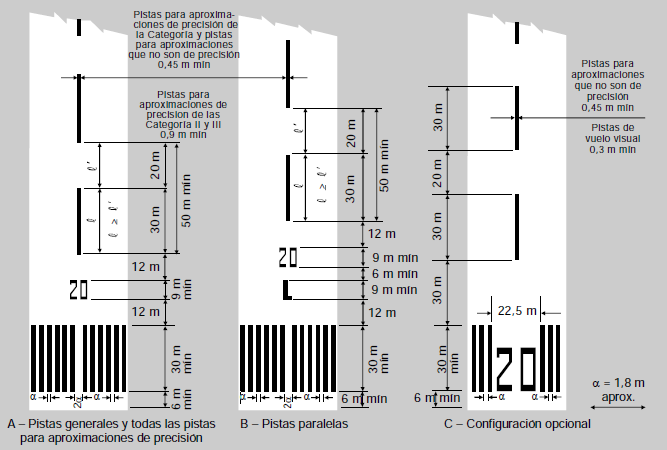
\includegraphics[clip, trim=0cm 0cm 0cm 0cm, width=0.911\textwidth]{./images/markings/centreline}
			\caption{Centreline according to ICAO's recommendations.} %nom de la figura
			\label{} %per denotar una referencia
		\end{figure}
	
		Due to the fact that the airport has two parallel runways, the model used will be the middle one. 
		
		The following figure attached will be shown as an example:
		
		\begin{figure}[H]
			\centering
			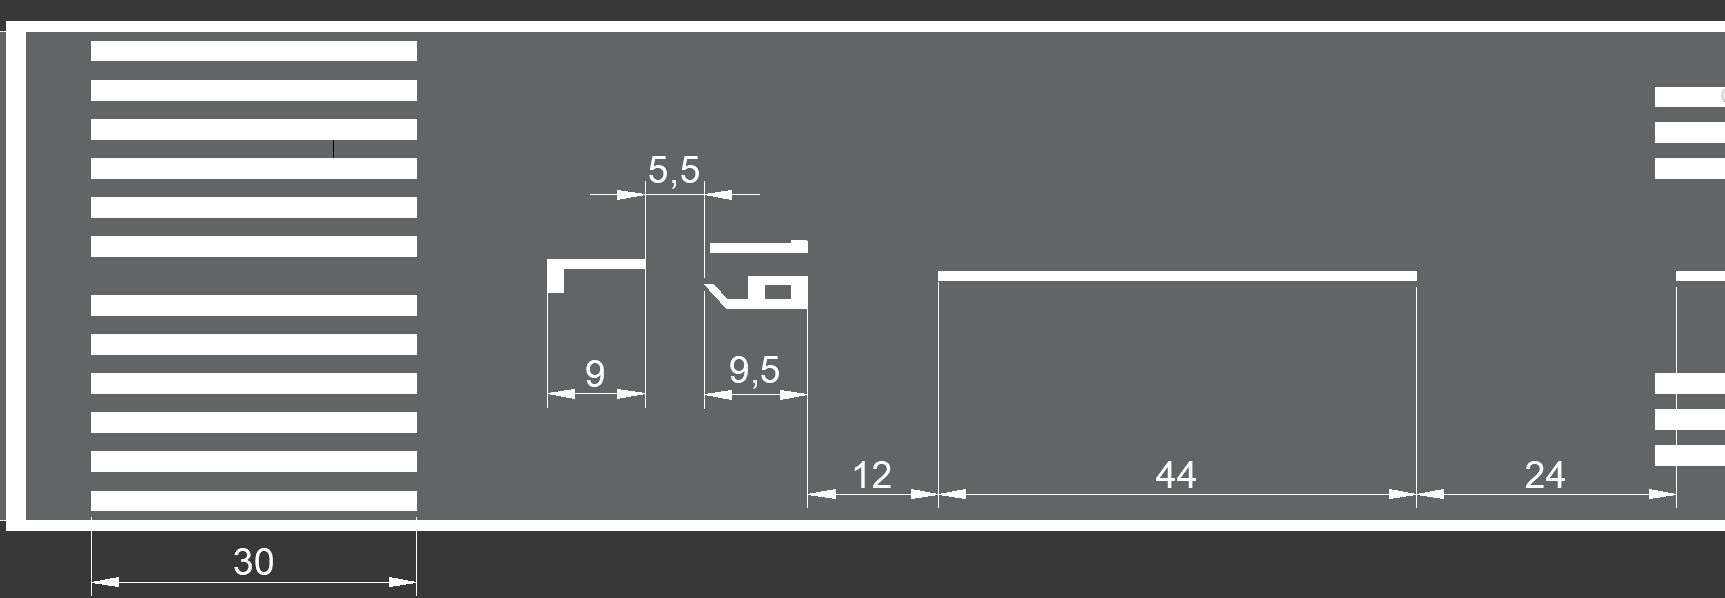
\includegraphics[clip, trim=0cm 0cm 0cm 0cm, 	width=0.911\textwidth]{./images/markings/centreexample}
			\caption{Centre line of the international runway.} %nom de la figura
			\label{} %per denotar una referencia
		\end{figure}
		
		\subsection{Runway's threshold markings}
		\paragraph{}The strips that indicate the start of the threshold will start at 6 m from the beginning of the threshold, and will contain 12 stripes, choosing the configuration specified in the Annex 14 part 5.2.4.6., including a minimum of 30m of length and 1,80m of width, with a separation of approximately 1,80m.
		
		\subsubsection{Arrows}
		\paragraph{}The runway's aiming point markings will be placed if the threshold is displaced from the runway extreme. As in the case of the Bekasi-East Jakarta both runways (4E and 4C) the threshold will be displaced, they are a must. They will be coloured in white.
		
		\begin{figure}[H]
			\centering
			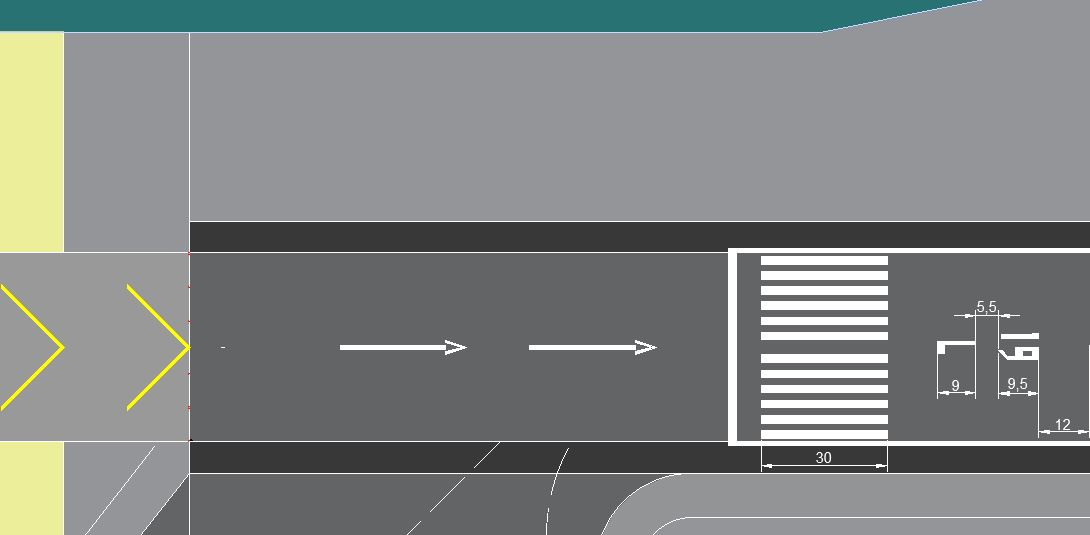
\includegraphics[clip, trim=0cm 0cm 0cm 0cm, 	width=0.911\textwidth]{./images/markings/arrows}
			\caption{Example of arrows pointing at the threshold.} %nom de la figura
			\label{} %per denotar una referencia
		\end{figure}
		
		\subsection{Runway's designation marking}
		\paragraph{}It will be placed in the threshold and in the case of Jakarta airport will be mandatory in all the cases as they all are paved. This designer will consist in two numbers referred to the azimuthal position. This number will be accompanied by a letter, indicating the order of appearance. 
		
		
		\subsection{Runway's aiming point markings}
		\paragraph{}As both runways meet the criteria, an aiming point is needed. The following table extracted from the annex 14 will show us which parameters should the aiming point mark have depending on the runway's category: 
		
		\begin{figure}[H]
			\centering
			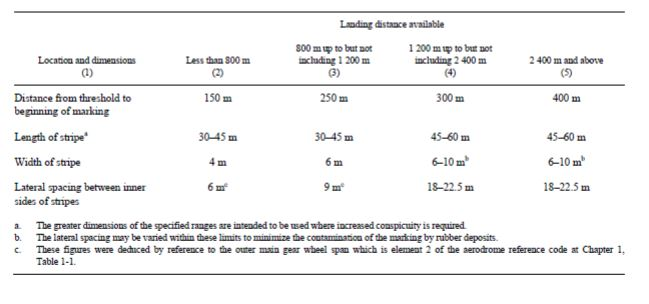
\includegraphics[clip, trim=0cm 0cm 0cm 0cm, 	width=0.8\textwidth]{./images/markings/aimpointtable}
			\caption{Table gathering all the aiming point marking parameters.} %nom de la figura
			\label{} %per denotar una referencia
		\end{figure}
		
		So, since both runways have a RFL higher than 2400m, the distance between the threshold and the start of the marking will be at 400 m, with a length of 60 m, a width of 10 m and a separation of 18 m. The following figure may serve as an example:
		
		\begin{figure}[H]
			\centering
			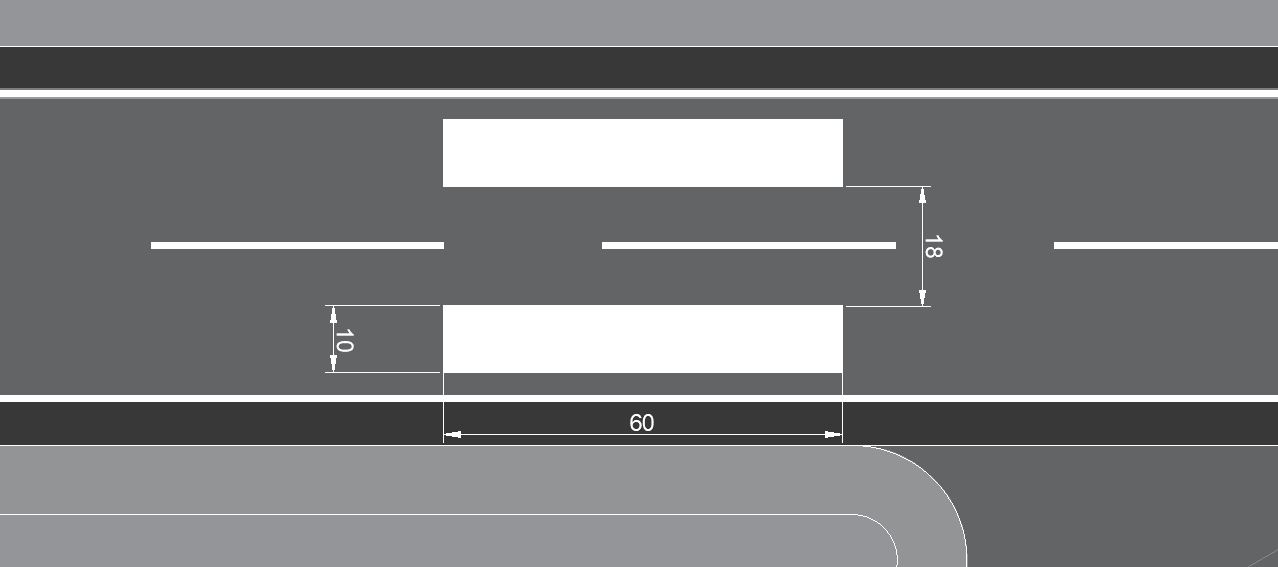
\includegraphics[clip, trim=0cm 0cm 0cm 0cm, 	width=0.911\textwidth]{./images/markings/aimpoint}
			\caption{Example of aiming point markings placed in runway 1.} %nom de la figura
			\label{} %per denotar una referencia
		\end{figure}
		
	\section{Taxiway's and holding position's markings}
		\subsection{Introduction}
		\paragraph{}Due to the fact that the airport being designed is a 4-type for both runways, the markings in the taxiways will be mandatory. The axis will be projected respecting the distances when curves appear and respecting the established hierarchy, that is to say, keeping in mind that they are subordinated to runways. The dimensions of this marking will be continuous and with 15cm of width at least, except in the event of an intersection.
		
		\subsection{Runway's entry holding position markings}
		The runway's entry holding position markings will be directly painted in the AutoCAD model following the regulations and recommendations stated in the annex 14.
				
		\subsection{Mandatory instruction markings}
		\paragraph{}If there is no possibility of positioning a sign with mandatory indications, this indication will be painted in the pavement. In the case of the type C runway, this signal will be centred in the middle of the centreline, interrupting it, whereas in the type F runway the signal will be placed twice on each side of the axis. 
		
		The characters will be painted in white with a red background and the height of the different characters should be of, at least, 4m.
		
		\begin{figure}[H]
			\centering
			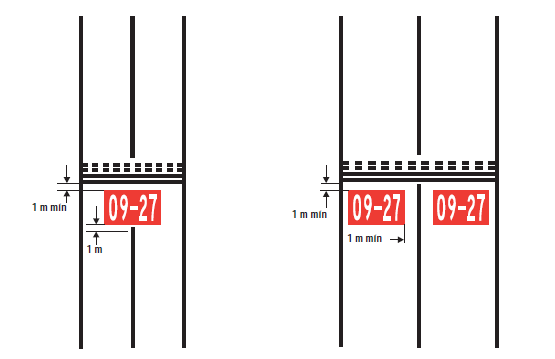
\includegraphics[clip, trim=0cm 0cm 0cm 0cm, 	width=0.911\textwidth]{./images/markings/mandatorymarks}
			\caption{Design used in order to define the mandatory instruction markings.} %nom de la figura
			\label{} %per denotar una referencia
		\end{figure}
	
		\subsection{Information markings}
		\paragraph{}Depending of the information given, the colours of the information markings will be:
		
		-	Yellow characters with black background if it gives emplacement information.
		
		-	Black background with yellow background if it gives direction or destiny information.
	
	\section{Apron's markings} 
		\subsection{Introduction}
		\paragraph{}They will include the identification number of every lot, with its guideline, alignment guide, stop line and departure line. The markings should be represented bearing in mind that the pilot should also be able to see the markings from the cabin. The guidelines should also be continuous with a width of, at least, 15cm, like the width of the alignment line in the final parking position.

		\subsection{Stand safety lines markings}
		\paragraph{}When considered necessary, the platform surface may include a safe separation distance between the different aircraft, such as wing tip margin lines. They will be continuous with a width of, at least, 10cm.

		
	
\chapter{Lights} % COMPROBAR TRADUCCIONES

	\section{Runway lights}
		\subsection{Approach lights}
		Due to the airport characteristics, it is defined as a precision approach runway II and III. According to that ICAO's classification, the starting point in order to design the approach lights is the rule 5.3.4.22. 
		
		The approach lighting system shall consist of a row of lights on the extended centre line of the runway,
		extending, wherever possible, over a distance of 900 m from the runway threshold. In addition, the system shall have two
		side rows of lights, extending 270 m from the threshold, and two crossbars, one at 150 m and one at 300 m from the threshold. Furthermore, the lights forming the centre line shall be placed at longitudinal intervals of 30 m with the innermost lights
		located 30 m from the threshold. 
		Moving into the point 5.3.4.24, the lights forming the side rows shall be placed on each side of the centre line, at a longitudinal spacing equal to that of the centre line lights and with the first light located 30 m from the threshold. Where the serviceability level of the approach lights specified as maintenance objectives in 10.5.7 can be demonstrated, lights forming the side rows may be placed on each side of the centre line, at a longitudinal spacing of 60 m with the first light located 60 m from the threshold. The lateral spacing (or gauge) between the innermost lights of the side rows shall be not less than 18 m nor more than 22.5 m, and preferably 18 m, but in any event shall be equal to that of the touchdown zone lights.
		
		Both points 5.3.4.25 and 5.3.4.27 are related to the crossbars. The crossbar provided at 150 m from the threshold shall fill in the gaps between the centre line and side row lights while the one provided at 300m shall extend on both sides of the centre line lights to a distance of 15 m from the centre line.
		
		The next image taken from annex 14 sums up all the points and requirements stated above: 
		
		\begin{figure}[H]
			\centering
			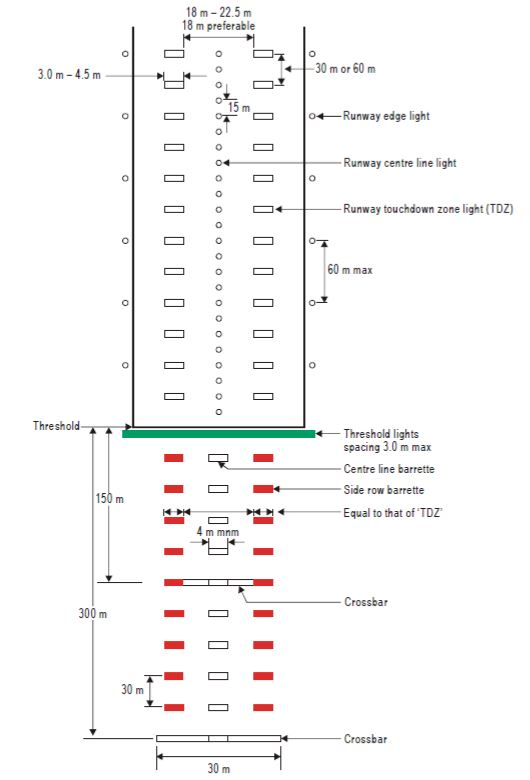
\includegraphics[clip, trim=0cm 0cm 0cm 0cm, width=0.45\textwidth]{./images/Annex14/approachlights}
			\caption{Schematic figure representing the approaching lights.} %nom de la figura
			\label{} %per denotar una referencia
		\end{figure} 
	
		\textit{Characteristics}
		
		According to ICAO, the centre line of a precision approach category II and III lighting system for the first 300 m from the
		threshold shall consist of barrettes showing variable white, except that, where the threshold is displaced 300 m or more, the
		centre line may consist of single light sources showing variable white. 
		
		Since the threshold of both runways is not displaced more than 300m, the centre line will consist of barrettes showing variable white. Those barrettes has to have a minimum length of 4m according to the article number 5.3.4.33.
		
		The side row shall consist of barrettes showing red. The length of a side row barrette and the spacing of its
		lights shall be equal to those of the touchdown zone light barrettes.
		
		\subsection{Approach slope indication systems}
		There are 4 types of approach slope indication systems: T-VASIS, AT-VASIS, PAPI AND APAPI. Depending on the system chosen, the design may change. In order to ease the maintenance costs and due to its easy design and installation, the system chosen is the PAPI.
		The recommendations and the rules that affect the PAPI and APAPI design range from the statement number 5.3.5.24 until the 5.3.5.41 inclusive.
		
		\textit{Description}
		
		The PAPI system shall consist of a wing bar of four sharp transition multi-lamp units
		equally spaced and the system shall be located on the left side of the runway unless it is physically impracticable to do so. 
		
		The wing bar of a PAPI shall be constructed and arranged in such a manner that a pilot making an approach
		will:
		
		a) When on or close to the approach slope, see the two units nearest the runway as red and the two units farthest from the runway as white.
		
		b) When above the approach slope, see the one unit nearest the runway as red and the three units farthest from the runway as white; and when further above the approach slope, see all the units as white.
		
		c) When below the approach slope, see the three units nearest the runway as red and the unit farthest from the runway as white; and when further below the approach slope, see all the units as red.
		
		\textit{Calculations}
		
		The location of the PAPI system should be the one that brings the highest compatibility with all the other visual and non-visual factors, considering facts such has the vertical distance of the pilot and the antenna of the planes that regularly use the runway. The distance is going to be equal to the medium length between the threshold and the beginning of the landing, adding a corrector factor due to the difference between the vertical length of the pilot eyes and the antenna. This factor can be obtained by multiplying the medium vertical distance between the pilot eyes and the antenna with the cotangent of the approximation angle. 
		
		Considering the landing distance of 400m and making use of the Annex 14, the factor of correction can be obtained considering a landing angle of 3\degree. The value obtained is 53,31m. Thus, the final PAPI location is 453,31m.
		
		In order to state the perpendicular distance between the PAPI and the runway, the following picture taken from ICAO's manual determines that value. 
		
		 \begin{figure}[H]
		 	\centering
		 	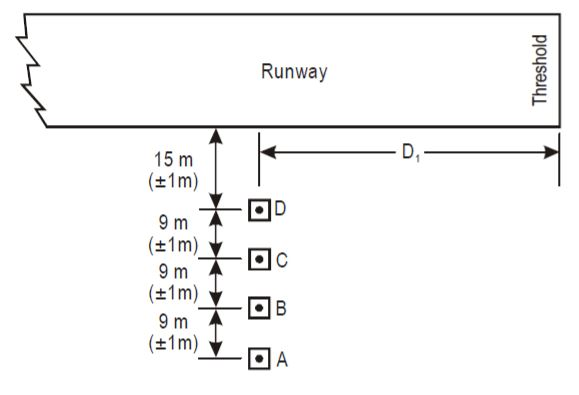
\includegraphics[clip, trim=0cm 0cm 0cm 0cm, width=0.75\textwidth]{./images/Annex14/PAPI}
		 	\caption{Vertical distance between the PAPI and the runway.} %nom de la figura
		 	\label{} %per denotar una referencia
		 \end{figure}
		
		In order to ensure the visibility of the PAPI system, an area empty of obstacles must be defined. The parameters that define this protective surface are gathered in the following table extracted from the Annex 14, chapter 5:
		
		\begin{figure}[H]
			\centering
			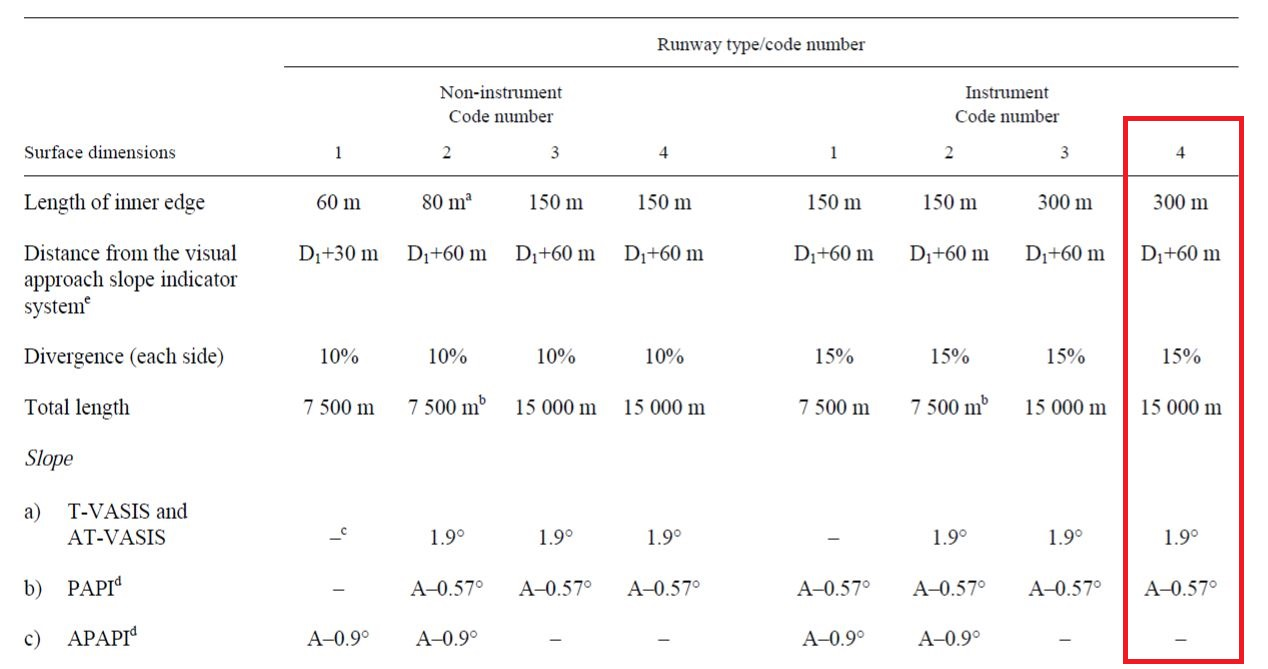
\includegraphics[clip, trim=0cm 0cm 0cm 0cm, width=1\textwidth]{./images/Annex14/SuperficiesPAPI}
			\caption{Dimensions and slopes of the obstacle protection surface.} %nom de la figura
			\label{} %per denotar una referencia
		\end{figure}
		
		The following figure extracted from the ICAO's manual can ease the understanding of the PAPI and its protection surface function:
		
		\begin{figure}[H]
			\centering
			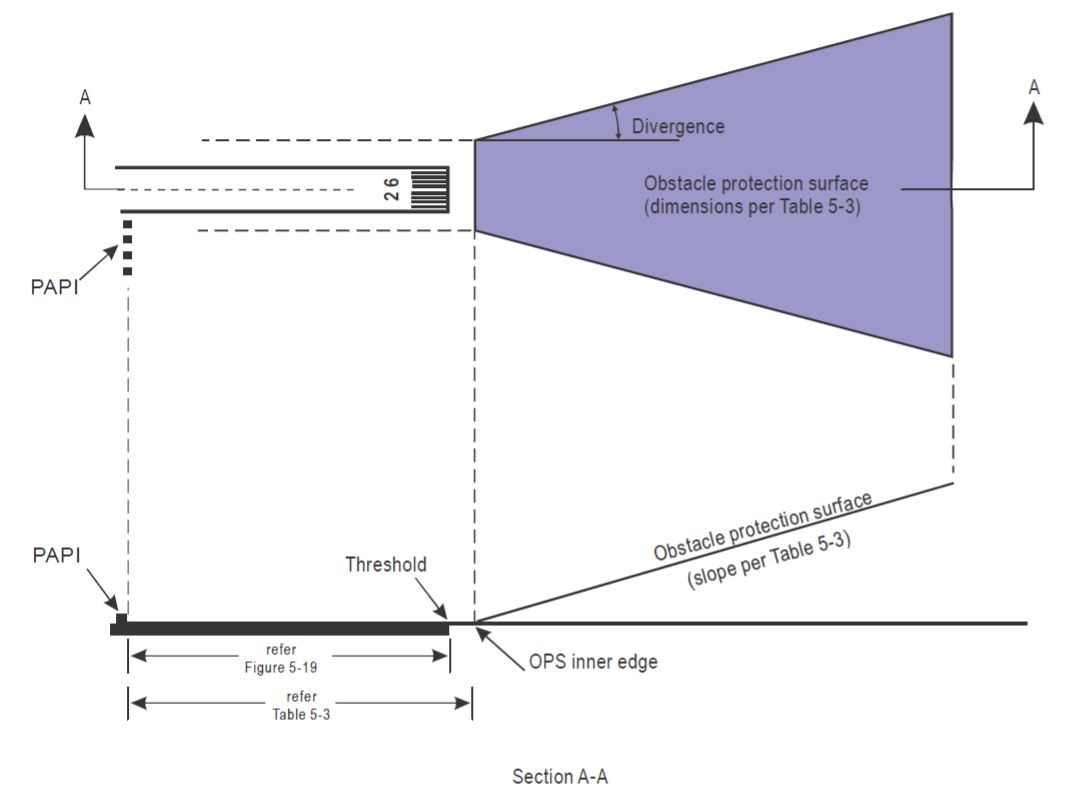
\includegraphics[clip, trim=0cm 0cm 0cm 0cm, width=1\textwidth]{./images/Annex14/PAPIScheme}
			\caption{Protection surface scheme and PAPI positioning.} %nom de la figura
			\label{} %per denotar una referencia
		\end{figure}
		
		\subsection{Runway threshold identification lights}
		The rules that regulate the runway threshold identification lights can be found on chapter 5.3.8 of the Annex 14. As a conclusion, the following statements define when should the threshold identification lights be included in the airport's installation:
		
		- In a visual approximation runway, when there are no more other reliable visibility aids. 
		
		- The threshold is permanently or temporary displaced from the beginning of the runway.
		
		Due to the fact that non of those requirements are meet, those lights have been discarded.
		 
		\subsection{Runway edge lights}
		Unlike the last set of lights, the runway edge lights are a must since the airport is expected to work during night time too. 
		
		Runway edge lights shall be placed along the full length of the runway and shall be in two parallel rows equidistant from the centre line. Their distance from the edge should not exceed the 3m. Furthermore, The lights shall be uniformly spaced in rows at intervals of not more than 60 m for an instrument runway. 
		
		Runway edge lights shall be fixed lights showing variable white except 600m before the end of the runway, in this case, may show yellow.
		
		\subsection{Runway threshold and wing bar lights} 
		Runway threshold will be provided since the runway is equipped with runway edge lights.
		
		\textit{Location}
		
		The threshold lights shall be placed in a row at right angles to the runway axis as near to the extremity of the runway as possible and, in any case, not more than 3 m outside the extreme. Furthermore, due to our approximation category, the lights will be uniformly spaced between the rows of runway edge lights at intervals of not more than 3 m.
		
		The use of wing bars is discarded since any of the runways is considered a visual approaching runway.
		
		\textit{Characteristics}
		
		Runway threshold and wing bar lights shall be fixed unidirectional lights showing green in the direction of approach to the runway.
		
		\subsection{Runway end lights}
		Following ICAO's legislations, runway end lights shall be provided for a runway equipped with runway edge lights. Their location is on a line as close as possible to the end of the runway, in any case, not more than 3 m outside the end.
		
		\textit{Characteristics}
		
		Runway end lights shall be fixed unidirectional lights showing red in the direction of the runway. The intensity and beam spread of the lights shall be adequate for the conditions of visibility and ambient light in which use of the runway is intended.
		
		The final configuration adding the contribution of the end lights and the threshold lights is the following:
		
		\begin{figure}[H]
			\centering
			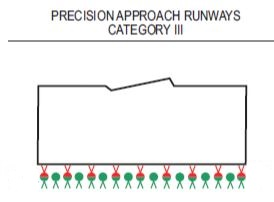
\includegraphics[clip, trim=0cm 0cm 0cm 0cm, width=0.65\textwidth]{./images/Annex14/endlights}
			\caption{Scheme showing the lights placed on the edge of the runway.} %nom de la figura
			\label{} %per denotar una referencia
		\end{figure}
		
		\subsection{Runway centre line lights}
		According to 5.3.12.11 the airports with precision approach runway of category II or III must provide centre line lights.
		
		 \textit{Location}
		 
		 Runway centre line lights shall be located along the centre line of the runway, except that the lights may be
		 uniformly offset to the same side of the runway centre line by not more than 60cm. The lights shall be located from the threshold to the end at longitudinal spacing of approximately 15m.
		
		\textit{Characteristics}
		
		Runway centre line lights shall be fixed lights showing variable white from the threshold to the point 900 m
		from the runway end; alternate red and variable white from 900 m to 300 m from the runway end; and red from 300 m to the
		runway end, except that for runways less than 1 800 m in length, the alternate red and variable white lights shall extend from
		the midpoint of the runway usable for landing to 300 m from the runway end.
		
		\subsection{Touchdown zone lights}
		\textit{Location}
		
		Touchdown zone lights shall extend from the threshold for a longitudinal distance of 900m and the longitudinal spacing between pairs of barrettes shall be either 30m or 60m.
		
		\textit{Characteristics}
		
		A barrette shall be composed of at least three white unidirectional variable lights with a spacing between the lights of not more than 1,5m. Its length will be higher than 3 and lower than 4,5m in order to successfully follow the recommendation 5.3.13.4.
			
		\subsection{Rapid exit taxiway indicator lights}
		A set of rapid exit taxiway indicator lights shall be located on the runway on the same side of the runway centre line as the associated rapid exit taxiway. In each set, the lights shall be located 2 m apart and the light nearest to the runway centre line shall be displaced 2 m from the runway centre line. Furthermore, rapid exit taxiway indicator lights shall be fixed unidirectional yellow lights, aligned so as to be visible to the pilot of a landing aeroplane in the direction of approach to the runway. 
		
		The following scheme simplifies the explanation shown above and can also be used to give an example of the application of the rapid exit taxiway indicator lights:
		
		\begin{figure}[H]
			\centering
			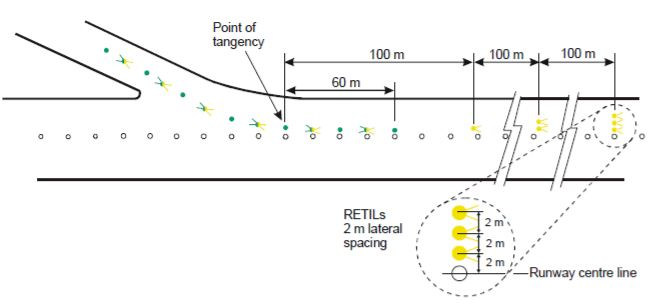
\includegraphics[clip, trim=0cm 0cm 0cm 0cm, width=0.85\textwidth]{./images/Annex14/rapidexittaxiways}
			\caption{Example of rapid exit runway lights.} %nom de la figura
			\label{} %per denotar una referencia
		\end{figure}
	
	\section{Taxiway lights}
		\subsection{Taxiway lights}
		\subsection{Taxiway lights for an exit taxiway}
		\subsection{Taxiway light for a rapid exit taxiway}
		\subsection{Taxiway edge lights}
		\subsection{Stop bar lights}
		\subsection{Intermediate holding point lights}
	
	\section{Apron lights}
		\subsection{Line and edge apron lights}
		\subsection{Projector based apron lighting}
		\subsection{Visual guidance system for parking}
		
		
		


\chapter{Signs}
	\section{Introduction}
	\paragraph{}Signs main objective is to give some information to the pilots about what lies ahead in order to guarantee the perfect organisation and efficiency of the aircraft trajectory while on taxiways. 
	
	The criteria used in order to dimension and calculate the position of each sign can be obtained from a table stated on the point 5.4 of the Annex 14.
	
	\begin{figure}[H]
		\centering
		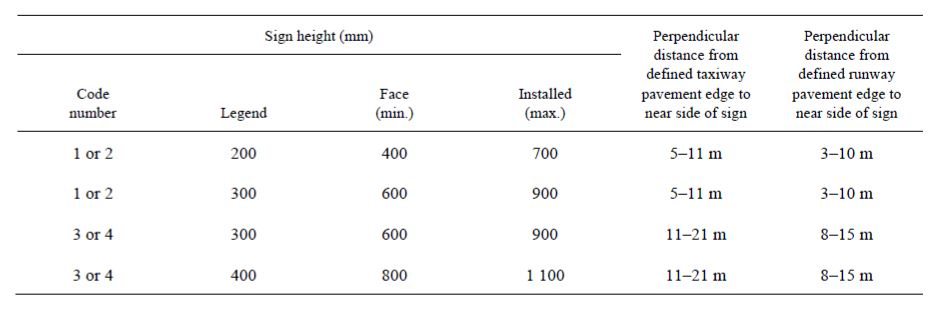
\includegraphics[clip, trim=0cm 0cm 0cm 0cm, width=0.95\textwidth]{./images/Annex14/signstable}
		\caption{Location distances for taxiing guidance signs.} %nom de la figura
		\label{} %per denotar una referencia
	\end{figure}

	Since the airport designed has a number reference of 4, the distance from the runway to the sign will be 12m and the distance from the taxiways will be 15m. Two different values have been chosen in order to help the pilots differentiate which sign are they looking at. 
	
	Another important aspect to be taken into account is the fact that all the signs will have inside illumination in order to allow the night time operations.
	
	\section{Mandatory instruction signs}
	\textbf{\textit{Application}}
	
	A mandatory instruction sign shall be provided to identify a location beyond which an aircraft taxiing or vehicle shall not proceed unless authorized by the aerodrome control tower. The signs included in this section are: designation signs, category I, II or III holding position signs, runway-holding position signs, road-holding position signs and NO ENTRY signs.
	
	\textbf{\textit{Location}}
	
	The location of each sign depend on the prohibition or the information they are giving:
	
	- A runway designation sign at a taxiway/runway intersection or a runway/runway intersection shall be located on each side of the runway-holding position marking facing the direction of approach to the runway.
	
	- A category I, II or III holding position sign shall be located on each side of the runway-holding position marking facing the direction of the approach to the critical area.
	
	- A NO ENTRY sign shall be located at the beginning of the area to which entrance is prohibited on each side of the taxiway as viewed by the pilot.
	
	\textbf{\textit{Characteristics}}
	
	A mandatory instruction sign shall consist of an inscription in white on a red background. Furthermore, in the specific case of inscription on a category I, II, III, joint II/III or joint I/II/III holding position sign shall consist of the runway designator, it must be followed by CAT I, CAT II, CAT III, CAT II/III or CAT I/II/III, as appropriate.
	
	\textbf{\textit{Examples}}
	
	Now that the mandatory instruction signs have been fully explained and defined, the next step is to place those signs in the airport. Some examples of the sign placed will be shown and explained:
	
	The NO ENTRY sing have been installed at the beginning of every rapid exit taxiway in both sides in order to aware the pilot that those taxiways are only allowed for the planes that land to exit the runway, entering the runway through a rapid exit way is strictly forbidden. The next figure shows the sign mentioned above:
	
	\begin{figure}[H]
		\centering
		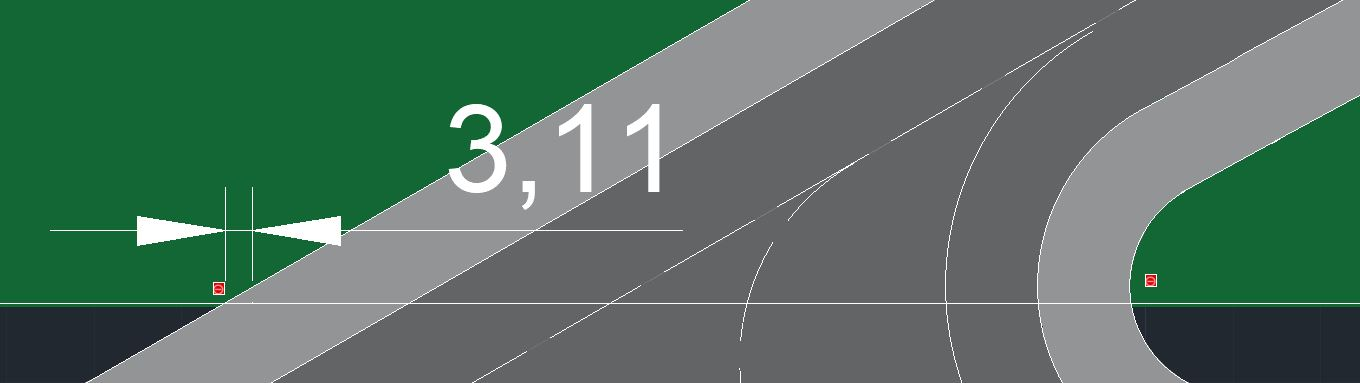
\includegraphics[clip, trim=0cm 0cm 0cm 0cm, width=0.95\textwidth]{./images/signsexamples/NOentrysign}
		\caption{No entry sign positioning and example.} %nom de la figura
		\label{} %per denotar una referencia
	\end{figure}
	 
	The following sign is used in order to indicate the holding position and has to be placed in both sides of the runway that leads to that critical area:
	
	\begin{figure}[H]
		\centering
		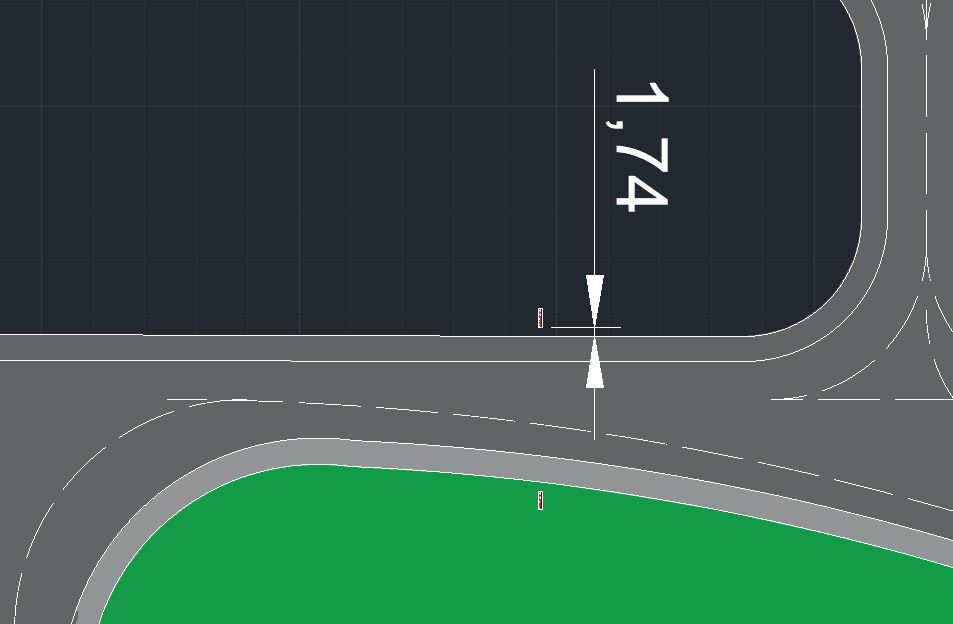
\includegraphics[clip, trim=0cm 0cm 0cm 0cm, width=0.95\textwidth]{./images/signsexamples/holdingposition}
		\caption{Holding positioning sign.} %nom de la figura
		\label{} %per denotar una referencia
	\end{figure}
	
	Since the sings can not be appreciated in the images due to the difference on the scale, some of the signs mentioned above will be shown in a bigger scale:
	
	\begin{figure}[H]
		\centering
		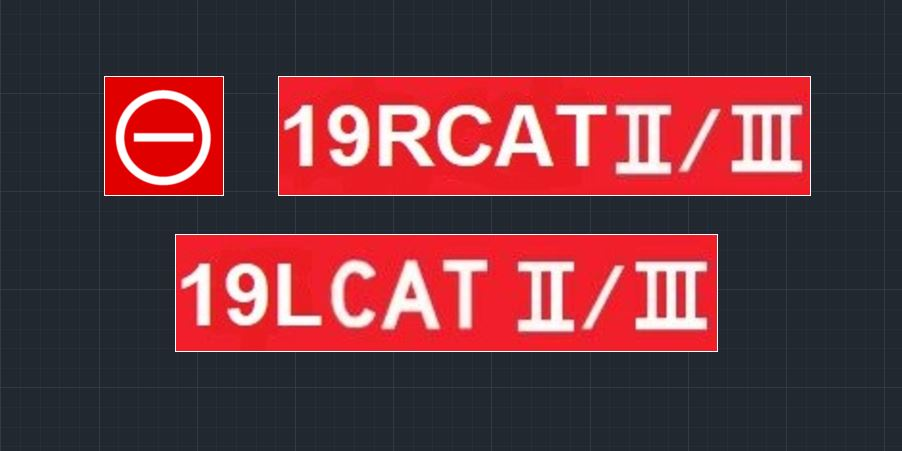
\includegraphics[clip, trim=0cm 0cm 0cm 0cm, width=0.8\textwidth]{./images/signsexamples/examples}
		\caption{Examples of the mandatory instruction signs used in the airport.} %nom de la figura
		\label{} %per denotar una referencia
	\end{figure}
	
	As it can be seen, both runways have their holding position in the direction 19, thus they have to be differentiated by an R (right) or L (Left), depending on the runway. Furthermore, the sign also displays information about the runway category. The other sign shown in the figure is the no entry sign.
	
	\section{Information signs}
	\textbf{\textit{Application}}
	
	An information sign shall be provided where there is an operational need to identify by a sign, a specific location, or routing information. Furthermore, information signs shall include: direction signs, location signs, destination signs, runway exit signs, runway vacated signs and intersection take-off signs.
	
	\textbf{\textit{Location}}
	
	Wherever practicable, the signs must be located on the left-hand side of the taxiway in accordance with table shown at the beginning of the section. Depending on the information sign, they get a different location:
	
	-At a taxiway intersection, information signs shall be located prior to the intersection and in line with the intermediate holding position marking. Where there is no intermediate holding position marking, the signs shall be installed at least 60 m from the centre line of the intersecting taxiway where the code number is 3 or 4, and at least 40 m where the code number is 1 or 2.
	
	- A runway exit sign shall be located prior to the runway exit point in line with a position at least 60 m prior to the point of tangency where the code number is 3 or 4, and at least 30 m where the code number is 1 or 2.
	
	\textbf{\textit{Characteristics}}
	
	A location sign shall consist of an inscription in yellow on a black background and where it is a stand-alone sign shall have a yellow border and the inscription on a runway exit sign shall consist of the designator of the exit taxiway and an arrow indicating the direction to follow.
	
	\textbf{\textit{Examples}}
	
	As for the mandatory instruction signs, now that the information signs have been defined, some examples will be given in order to ease the understanding of their function: 
	
	The first signs that will be exemplified will be the available runway length information signs. Those signs are placed in the entrance to the runway and give the available length that the aircraft has in order to perform the takeoff. Generally, they are only given in one side of the intersection. 
	
	\begin{figure}[H]
		\centering
		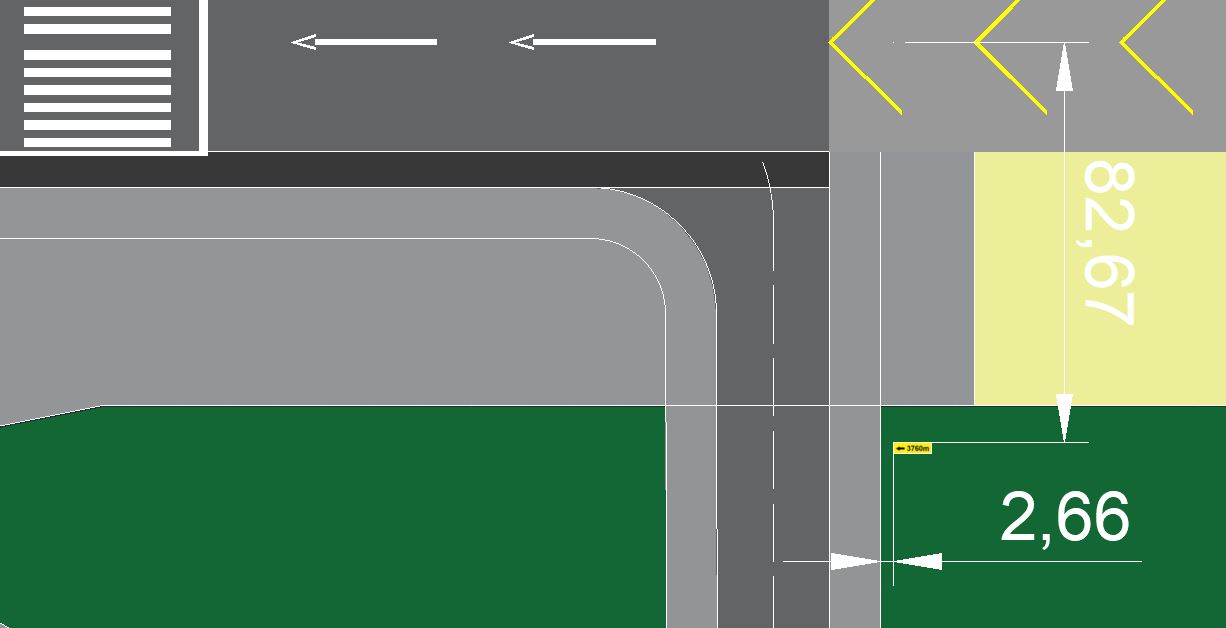
\includegraphics[clip, trim=0cm 0cm 0cm 0cm, width=0.8\textwidth]{./images/signsexamples/TODAsign}
		\caption{Available length information sign positioning.} %nom de la figura
		\label{} %per denotar una referencia
	\end{figure}

	The next signs that will also be explained are the ones that show information about the exit runway letter after landing. Each exit has assigned a different letter, thus there is one sign for each exit and rapid exit. All the signs will be place at the same distance from the runway. 
	
	\begin{figure}[H]
		\centering
		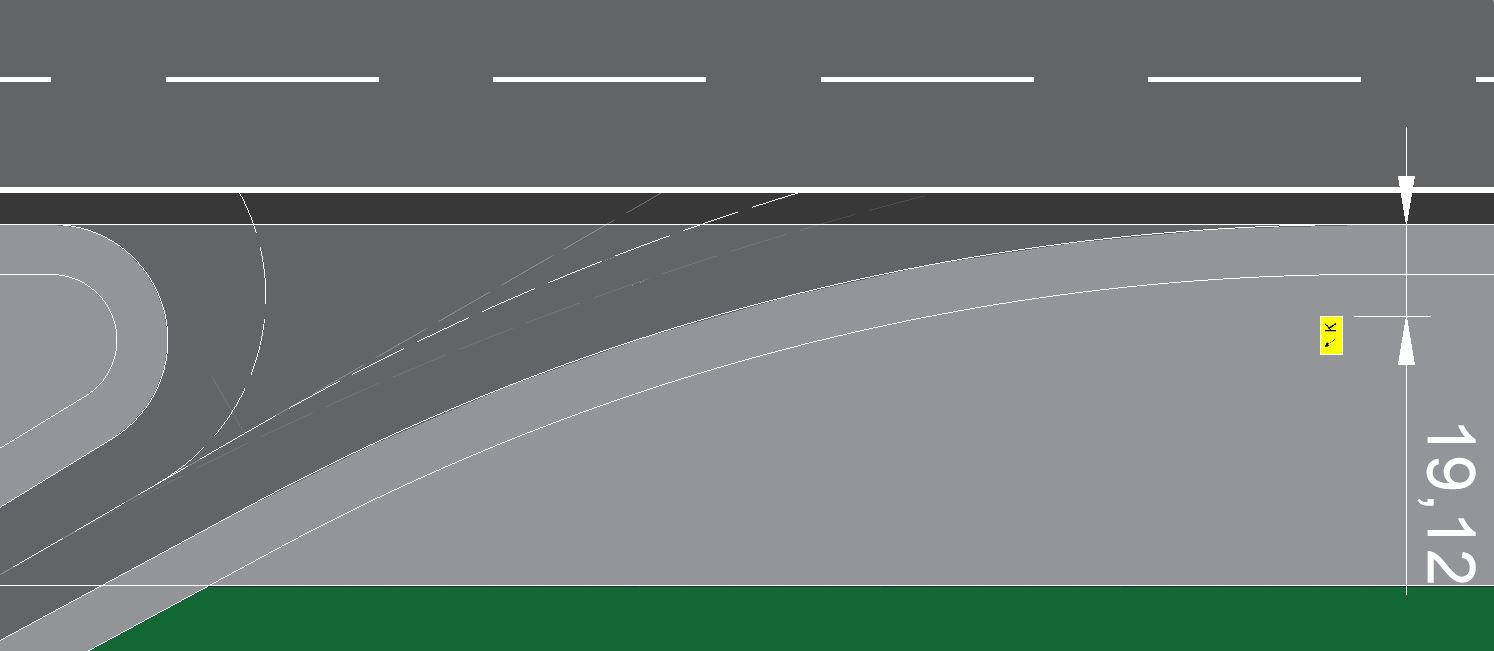
\includegraphics[clip, trim=0cm 0cm 0cm 0cm, width=0.8\textwidth]{./images/signsexamples/exitexample}
		\caption{Exit runway sign distances and positioning.} %nom de la figura
		\label{} %per denotar una referencia
	\end{figure}

	Finally, an image with some of the informative sign will be shown:
	
	\begin{figure}[H]
		\centering
		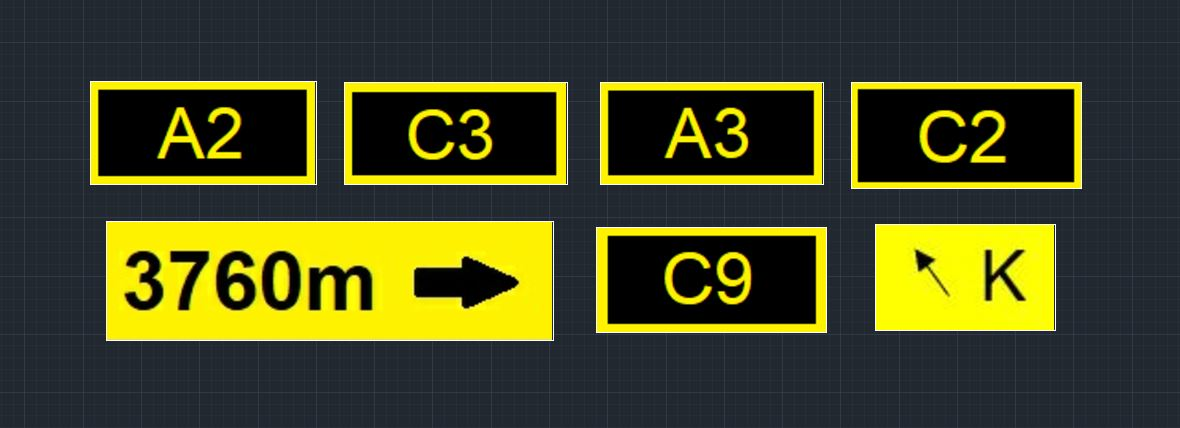
\includegraphics[clip, trim=0cm 0cm 0cm 0cm, width=0.8\textwidth]{./images/signsexamples/exempleinf}
		\caption{Exit runway sign distances and positioning.} %nom de la figura
		\label{} %per denotar una referencia
	\end{figure}
	
	The signs with black background and a yellow rectangle are the signs used in order to inform the pilot which is his current location. 
	

	
\chapter{High-voltage electrical system}

	\section{Electrical system general design}
	
	\section{Connection sub-stations}
	
	\section{Electric powerplant}
	
	\section{Electrical transformation center}
	
	\section{Channeling and distribution of the electrical system}
	
\chapter{Medium voltage electrical system}

	\section{Beacon circuits}
	\paragraph{} In series circuit is selected for beacon circuits, illustrated in figure \ref{series}. This option is chosen because its advantages.
	\begin{figure}[H]
		\centering
		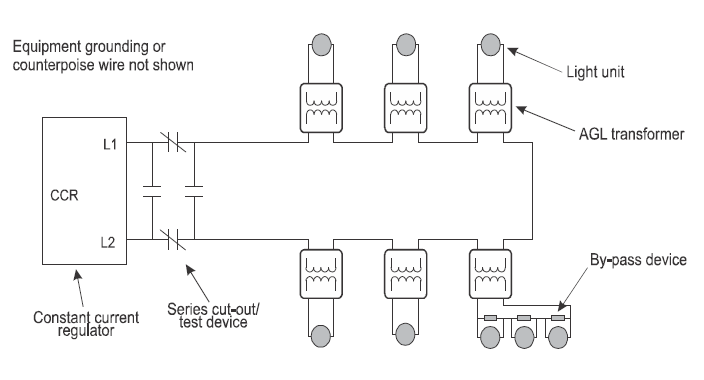
\includegraphics[clip, trim=0cm 0cm 0cm 0cm, width=0.7\textwidth]{./images/electric/series}
		\caption{Series lighting circuit.}
		\label{series}
	\end{figure}

	The constant current regulators of a series circuit, maintain a constant current independent of the load on the circuit. Thus, the same current will flow in a long circuit as in a shorter circuit and will remain the same even if some of the lamps fail. A short circuit across the output of a constant current regulator is a no-load condition and an open circuit is an overload. In a simple direct-connected series circuit, a lamp failure causes an open circuit; hence, it is necessary to provide an aerodrome ground lighting (AGL) transformer, as part of the circuit design, to maintain continuity of the circuit with lamp failure. Where a single transformer is used to supply several light units, as shown in Figure \ref{series}, a by-pass device is incorporated to ensure continuity on the secondary side.
	
	\subsection{Interleaving}
	\paragraph{} As a further means of assuring availability in case of failure, arrangement is made to enable switching to a spare regulator, as shown in Figure \ref{interleaved}. This method may be used where the regulator consists of the regulating component and input/output transformers. In the case of regulators that consist of only the regulating component, a rack mounted or plug-in design is used and availability is achieved by use of a spare regulator, Figure \ref{spare}, that can be readily installed in
	place of the failed regulator.
	
	\begin{figure}[H]
		\centering
		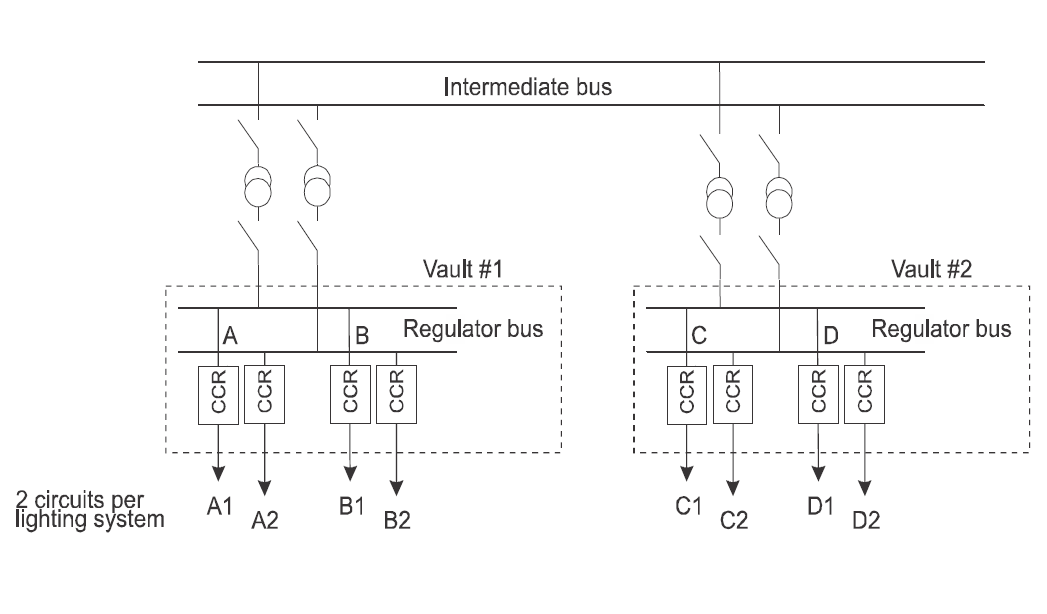
\includegraphics[clip, trim=0cm 0cm 0cm 0cm, width=0.8\textwidth]{./images/electric/interleaved}
		\caption{Provision of interleaved circuits.}
		\label{interleaved}
	\end{figure}

	\begin{figure}[H]
		\centering
		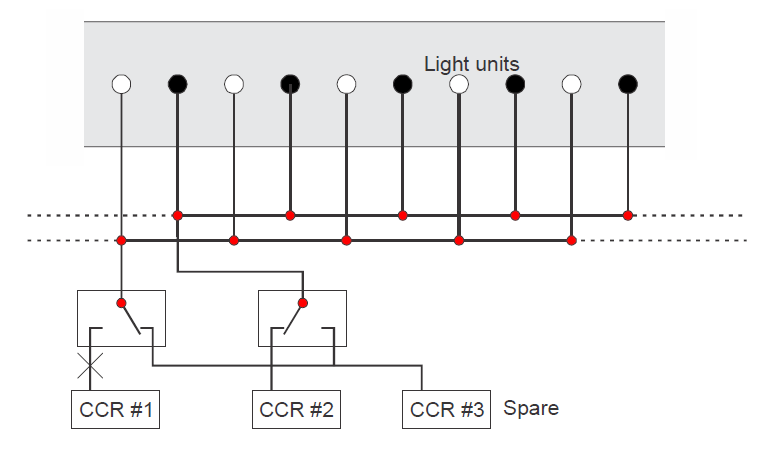
\includegraphics[clip, trim=0cm 0cm 0cm 0cm, width=0.7\textwidth]{./images/electric/spare}
		\caption{Use of a spare regulator.}
		\label{spare}
	\end{figure}
	
	
		\subsection{Runway centreline and touchdown lighting systems}
		\paragraph{} Annex 14, Volume I, requires that runway centreline lights show variable white to a distance of 900 m from the threshold, then alternating variable white and red from 900 m (or from the mid-point of the runway) to 300 m from the runway end after which only red is shown to the pilot. Figure \ref{rnwCentre} illustrates the interleaving for the first white only portion of the system. Similar interleaving would be used for the final all red portion.		
		
		\begin{figure}[H]
			\centering
			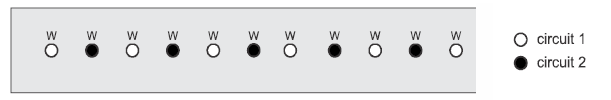
\includegraphics[clip, trim=0cm 0cm 0cm 0cm, width=0.7\textwidth]{./images/electric/rnwCentre}
			\caption{Runway centreline.}
			\label{rnwCentre}
		\end{figure}
		
		Interleaving to preserve spacing, Figure \ref{spacing}, is selected for the coded white/red portion of the system. This configuration, does not preserve the coding (with circuit failure the lights are either all red or all white), but does maintain an acceptable spacing for provision of a pattern of lights for centreline guidance (the spacing is doubled with circuit failure).
		
		\begin{figure}[H]
			\centering
			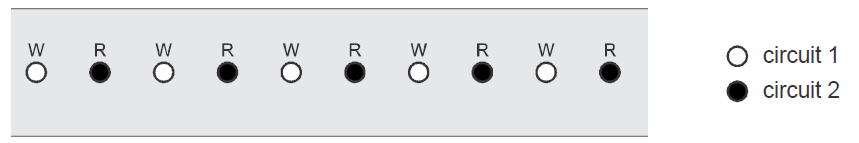
\includegraphics[clip, trim=0cm 0cm 0cm 0cm, width=0.7\textwidth]{./images/electric/spacing}
			\caption{Interleaving to preserve spacing.}
			\label{spacing}
		\end{figure}
	
		Figure \ref{touchdown} also illustrates the interleaving of runway touchdown zone lights. In this case three circuits will be used to preserve longitudinal spacing in case of one circuit failure.	
		\begin{figure}[H]
			\centering
			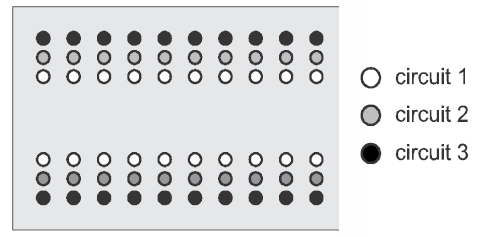
\includegraphics[clip, trim=0cm 0cm 0cm 0cm, width=0.7\textwidth]{./images/electric/touchdown}
			\caption{Interleaving by horizontal lines with three circuits.}
			\label{touchdown}
		\end{figure}
		
		
		\subsection{Taxiway centreline lighting system}
		\paragraph{} Taxiway centreline lighting circuits will be interleaved on those parts of the taxiway system that are considered as essential in category II/III conditions but, for economic reasons, a single circuit may be used for other taxiways.
		
		Three circuits for interleaving procedure will be use, figure \ref{inter3}. Because there is a lot of operations movement, is essential to preserve both spacing and colour, to reduce the chance of pilots getting lost.
		
		\begin{figure}[H]
			\centering
			\includegraphics[clip, trim=0cm 0cm 0cm 0cm, width=0.7\textwidth]{./images/electric/inter3}
			\caption{Interleaving to preserve both spacing and colour.}
			\label{inter3}
		\end{figure}
		
		\subsection{Stop bar electrical circuit}
		\paragraph{} Stop bars will be controlled independently of each other and of the taxiway centreline lights. The electrical circuits will be interleaved so that all of the lights of a stop bar will not fail at the same time.
		
		\subsection{Approach lighting system}
		
			\subsubsection{Visual approach, PAPI electrical circuit}
			\paragraph{} Visual approach slope indicator systems will have two circuits per runway end because they are operated with an ILS system.
			
			A full PAPI or T-VASI will be installed on both sides of the runway, the power to all light units on one side of the runway will be supplied by the same circuit. This arrangement ensures that should one circuit fail a complete pattern will be retained on the other side of the runway.
					
			
			\subsubsection{Precision approach}
			\paragraph{} Precision approach interleaving implemented are summarized on figure \ref{pApp}.
			\begin{figure}[H]
				\centering
				\includegraphics[clip, trim=0cm 0cm 0cm 0cm, width=0.8\textwidth]{./images/electric/pApp}
				\caption{Precision approach lighting system interleaving.}
				\label{pApp}
			\end{figure}
			
		\subsection{Runway holding position signs}
		\paragraph{} Runway holding position signs will be installed such that separate circuits are used for the signs on each side of the taxiway.
		
		\subsection{RETIL electrical circuit}
		\paragraph{} The rapid exit taxiway indicator lights (RETIL) system is composed of a pattern of in-pavement fixtures used to indicate the approach to a runway exit. In as much as the system has a small quantity of fixtures and each is necessary for the distance coding, the RETIL system is not provided with interleaving but has a single circuit that is fed from a separate constant current regulator.
		
		Failure of one light within a barrette results in a malfunction of the system. Therefore, the system will be provided with an automatically turn off the entire system circuit, if there is a loss of a single light unit.
				
		
	\section{Constant current regulators}
	\paragraph{} The electrical power for the aerodrome ground lighting circuits (series circuit) is supplied by constant current regulators (CCRs) because this facilitates constant light output over long distances, as is the case for aerodrome runways. The regulators are designed to produce a constant current output that is independent of variations in the circuit load and input voltage of the power source. They are also designed to provide two or more output currents when
	dimming of the lights is required. 
	
	Projected airport will have two CCRs in order to power the aerodrome ground lighting circuit. Each one, powers the lights of half of each runway.
	
	
	\section{Wire channelling}
	\paragraph{} Primary beaconing 5KV grid and low tension circuit will be installed in  ducts encased in concrete, figure \ref{concrete}. All ducts installed in concrete encasement will be placed on a layer of concrete not less than 75 mm thick.
	
	Flared ends of ducts or couplings will be installed flush with the concrete encasement or inside walls of manholes or handholes. Interlock spacers will be used at not more than 1.5 m spacing to ensure uniform spacing between ducts. Joints in adjacent ducts will be staggered a minimum of 600 mm apart and will be made waterproof prior to concreting. Concrete-encased duct will be installed so that the top of the concrete envelope or conduit is not less than 450 mm below the stabilized base course where it is installed under roadways, railroads, runways, taxiways, other paved areas and ditches, and not less than 450 mm below the finished grade elsewhere. Counterpoise wires are provided as required.
	
	\begin{figure}[H]
		\centering
		\includegraphics[clip, trim=0cm 0cm 0cm 0cm, width=1.1\textwidth]{./images/electric/concrete}
		\caption{Concrete encased duct bank.}
		\label{concrete}
	\end{figure}
	
	In order to make easier the maintenance and installation, these connections will be simple and when possible in straight lines. When there is a change in direction, a manhole or hand-hole will be installed.
	
	

\chapter{Aeronautical limitation surfaces}

	\section{Physical limitation surfaces}
	\paragraph{} As runaway 1 and 2 are both classified as category 4, the dimensions of the Aeronautical Servitudes are the same for both. Using the defined OBSTACLE LIMITATION SURFACES (figure \ref{servitudeMap}), on ATTACHMENT B of \cite{Standards2016}.
	
	\begin{figure}[H]
		\centering
		\includegraphics[clip, trim=0cm 0cm 0cm 0cm, width=\textwidth]{./images/servidumbres/servitudeMap}
		\caption{Obstacle Limitation Surface model.}
		\label{servitudeMap}
	\end{figure}

	The servitudes for each runway are determined on the following table and represented on figure \ref{3Dservidumbres}.
	
	%AFEGIR TAULA
	\begin{longtable}[htb]{@{}lr@{}}
		\toprule[3pt]
		\multicolumn{2}{c}{\textbf{\large RUNWAYS 1 \& 2  } }\\ \midrule[2pt]
		\multicolumn{2}{c}{\textbf{Conic} }\\
		\midrule[0.5pt]
		Slope & 5\%\\
		Height & 100m\\
		\midrule[2pt]
		\multicolumn{2}{c}{\textbf{Internal Horizontal} }\\
		\midrule[0.5pt]
		Height & 45m\\
		Radius & 4.000m\\
		\midrule[2pt]
		\multicolumn{2}{c}{\textbf{Internal Approximation} }\\
		\midrule[0.5pt]
		Width & 120m\\
		Distance from edge & 60m\\
		Length & 900m\\
		Slope & 2\% \\
		\midrule[2pt]
		\multicolumn{2}{c}{\textbf{Approximation} }\\
		\midrule[0.5pt]
		Inner band length & 300m\\
		Distance from edge & 60m\\
		Divergence & 15\% \\
		\midrule[0.5pt]
		\multicolumn{2}{c}{First section} \\
		\midrule[0.5pt]
		Length & 3.000m\\
		Slope & 2\%\\
		\midrule[0.5pt]
		\multicolumn{2}{c}{Second section} \\
		\midrule[0.5pt]
		Length & 3.600m\\
		Slope & 2.5\%\\
		\midrule[0.5pt]
		\multicolumn{2}{c}{Horizontal section} \\
		\midrule[0.5pt]
		Length & 8.400m\\
		Total length & 15.000m\\
		\midrule[2pt]
		\multicolumn{2}{c}{\textbf{Transition} }\\
		\midrule[0.5pt]
		Slope & 14.3\%\\
		\midrule[2pt]
		\multicolumn{2}{c}{\textbf{Inner Transition} }\\
		\midrule[0.5pt]
		Slope & 33.3\%\\
		\midrule[2pt]
		\vspace{5cm}&\vspace{5cm}\\
		\midrule[2pt]
		\multicolumn{2}{c}{\textbf{Interrupted Landing} }\\
		\midrule[0.5pt]
		Inner band length & 120m\\
		Distance from edge & 1800m\\
		Divergence & 10\%\\
		Slope & 3.3\%\\
		\midrule[2pt]
		\multicolumn{2}{c}{\textbf{Take-off Climb} }\\
		\midrule[0.5pt]
		Inner band length & 180m\\
		Distance from edge & 60m\\
		Divergence & 12.50\%\\
		Final width & 1.200m\\
		Length & 15.000m\\
		Slope & 2\% (a)\\
		\bottomrule[3pt]
		\caption{Runways 1 \& 2 servitudes. (a): It is recommended to limit the presence of new objects to a surface with a slope of 1.6\%}
	\end{longtable}
	
	The obstacle free surfaces are the same for the two runways, since they are both of category III. All the data in the table is required in order to achieve this category of precision approximation.
	
	After study of the terrain, it is concluded that there are no obstacles in inside the surfaces. The control tower is below the conic surface as well.
	
	
	\begin{figure}[H]
		\centering
		\includegraphics[clip, trim=0cm 0cm 0cm 0cm, width=0.45\textwidth]{./images/servidumbres/3Dservidumbres}
		\caption{Servitudes 3D view.}
		\label{3Dservidumbres}
	\end{figure}

	
	\section{ILS limitation surfaces}
		\section{Localizer limitation surfaces}
		\section{Gliding trajectory protection limitation surfaces}


% BIBLIOGRAPHY

% styles:
%	abbrv   : [#] Initial. Surname (pages and vol. abbrev.)
% 	acm     : [#] Surname, Initial. (sc)
%	alpha   : [Abrev.yy] Name Surname
%	apalike : [Surname, yyyy] Surname, Initial 
%	ieeetr  : [#] Initial. Surname (pages and vol. ext.)
%	plain   : [#] Name Surname
%	siam    : [#] Initial. Surname (sc)
%	unsrt   : [#] Name Surname

\nocite{*}
\bibliographystyle{IEEEtran}
\bibliography{IEEEabrv,PROYECTO_AEROPUERTOS-LADO_AIRE} 

\end{document}